%!TEX root = ../../thesis.tex

\graphicspath{{Chapters/litreview/figures/}}
\chapter{Literature Review}

\section{Introduction}
Having explored common computer vision datasets and covered the fundamentals, design, and usage of neural networks,
 moving on to more advanced material is now possible. \added{In this chapter, the \textit{taxonomy} of network design
will first be covered, defining what constitutes a neural architecture and why it is such a broad problem.} Next,
the history of convolutional neural network
design will be covered, investigating the landmark results and principles that have been uncovered in the 10 years since
convolutional neural networks first demonstrated their immense computer vision potential. From this foundation of the
cutting-edge of human design, this thesis will then look at algorithmic network design, examining the different approaches that have been
tried to automatically design networks more complex and more powerful than anything seen before. However, this power comes
with significant caveats and shortcomings, which are then explored in the third section of this chapter. Here,
the flaws and fundamental scientific unsoundness of a subset of these algorithms is discussed, as well as the lessons that can
be learned from these flaws.

\section{On Neural Architectures}
\added{
When defining more complex networks such as CNNs or RNNs, the operations listed in Chapter\ref{chapter:background} such
    as convolutions or poolings can
be put together in any order, and the data can be defining to flow through these components in any number of ways. A good analogy
is that of a circuit; we have various components (resistors, capacitors, inductors, diodes, transistors)
that are be connected by wires, and finding novel combinations and connectivities of those components has constituted
the majority of human technical discovery in the last century or so. Neural architectures are very similar; we have
a huge gamut of components (each with a variety of possible specifications, like kernel size or output dimensionality),
each of which can be chosen an arbitrary number of times, and then these components can all be linked up in an infinite
number of ways. One way to conceptualize this infinite design space is that of graphs as in Figure~\ref{fig:arch_graph}, where nodes represent data aggregation
    (i.e., summation or concatenation) and edges represent data modification via operations like convolutions or poolings. }

\begin{figure}
    \centering
        \begin{subfigure}{.3\textwidth}
            \centering
            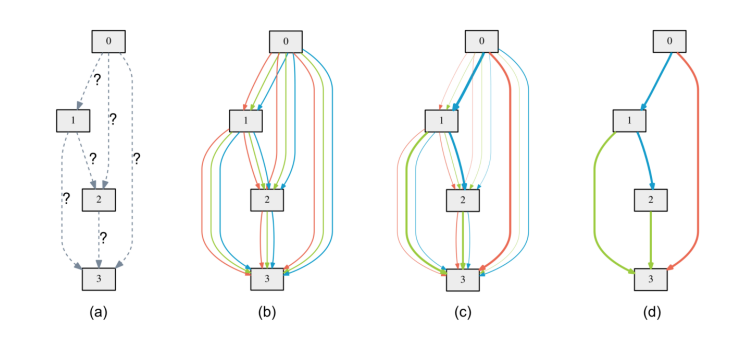
\includegraphics[trim={10cm .7cm 0 0cm},clip]{DARTS_cell}
        \end{subfigure}
        \begin{subfigure}{.3\textwidth}
            \centering
            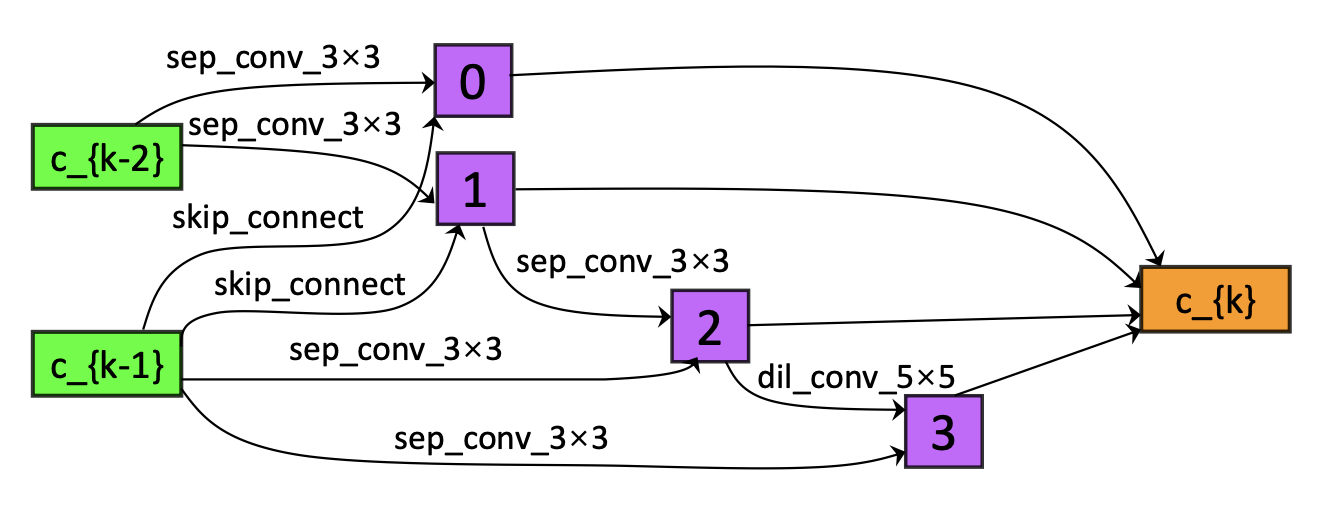
\includegraphics[width=1.3\textwidth]{pcdartscell}
        \end{subfigure}
        \begin{subfigure}{.3\textwidth}
            \centering
            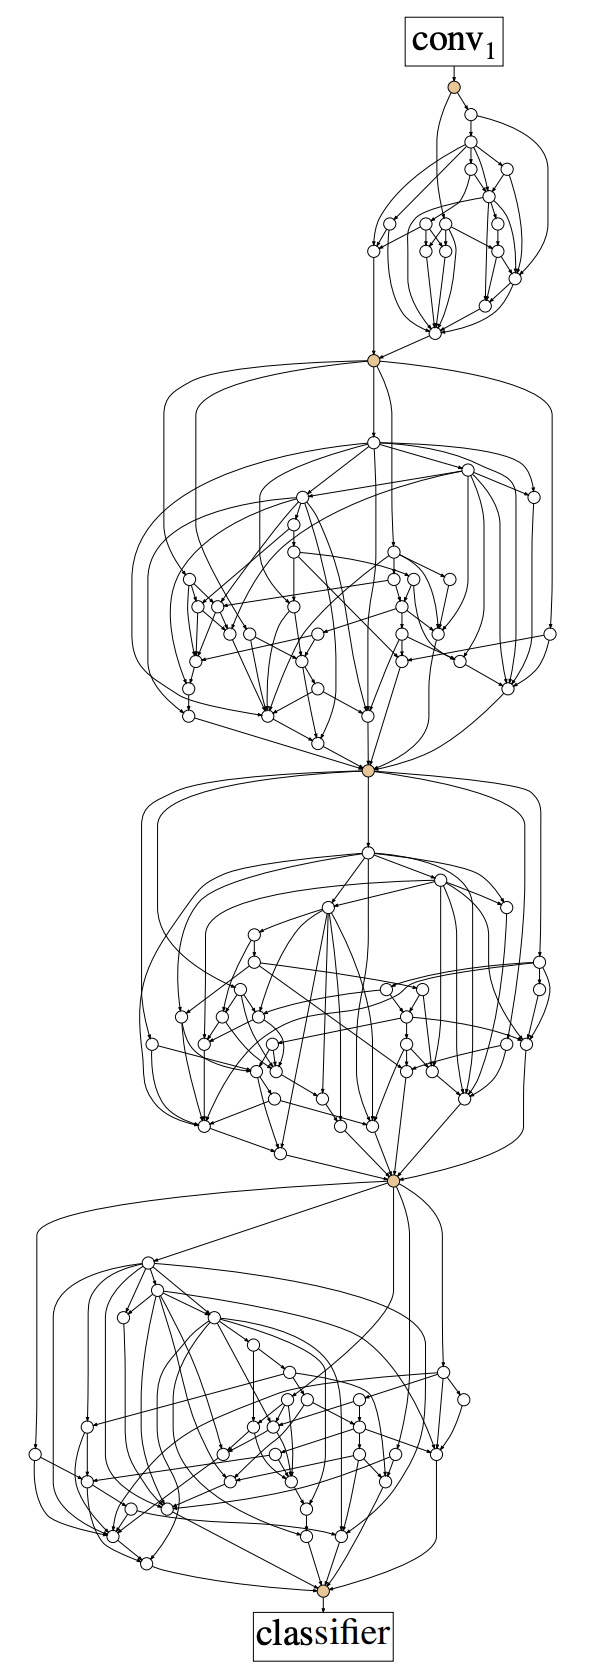
\includegraphics[height=15em]{random_wiring2}
        \end{subfigure}
    \caption[Graph representations of architectures]{Various graph representation of architectures, from~\cite{liu2018,xu2020,xi2019}.}
    \label{fig:arch_graph}
\end{figure}

\added{
    In this representation, any arbitrary graph can be converted into a neural architecture simply by defining which aggregations
    happen at each node and which operations lie along each edge. The problem of architecture design stems from the fact that the
        particular choice of graph, of operation-edge assignment,
    of nodal aggregation, all affect the final efficiency and performance of the network on the chosen task. As such,
    finding a good design is crucial to finding effective models.}
\added{However, picking a good model in this infinite design space
of all possible graphs can feel like finding a needle in an infinite haystack, and as such it is common to limit the
the network design space into a \textit{search space}: the set of all possible models that are eligible to be designed by a
particular algorithm or search strategy. The search space places constraints on the possible models that may be
designed, for example, that graphs must be acyclic or that only one edge can connect any two nodes. Meanwhile,
    textit{search algorithms} are methods that pick a specific architecture from within the set defined by a search space.}

\added{Since network design is such a crucial factor in its efficacy, the history of deep learning advances is one of design advances.
This chapter will explore both the manual design leaps that brought the field to where it is today, as well as the automated
design methods that seek to find needles within the infinite haystack for us.
}

\section{Manually Designed Convolutional Neural Nets}
\subsection{AlexNet}
Prior to early 2010s, convolutional neural networks were mostly a computational novelty. They had shown promising results on
small problems such as MNIST~\citep{lecun1989}, but were so computationally expensive to train that they were infeasible to use
for larger problems like CIFAR-10 or ImageNet. However, in 2012~\citeauthor{kriv2012}
published \hyperlink{cite.kriv2012}{``ImageNet Classification with Deep Convolutional Neural Networks''} which realized the potential that
graphics processing units or GPUs had to radically speed up training. The insight was thus: GPUs are designed to perform large scale
matrix and vector computations very efficiently in parallel, which are the exact computations which comprise the majority
of tensor operations within deep learning models. \citeauthor{kriv2012} wrote GPU implementations
of the operations necessary to run a convolutional neural network, dramatically speeding up the training of their model.
Their model had 60 million trainable parameters between five convolutional layers and three fully-connected layers, distributed
across two GPUs via a specialized parallel network architecture.
This was necessary to compensate for the relative lack of memory on GPUs at the time, and thus one GPU was tasked with
handling the top of the image and one the bottom, with data shared between
the two at limited points through the model.

Within this architecture they introduced ``new and unusual'' components to the convolutional neural network. The first of the
components were ReLU nonlinearities, which were added due to their desirable non-saturating quality as
described in Chapter 1. Next was local normalization, which served to normalize values over a local spatial area. The authors
acknowledge that while ReLU nonlinearities do not explicitly require normalization of their values in the same way that
saturating functions do, normalization still provided boosts to the model's test accuracy. Finally, they used overlapping
pooling, which was simply a pooling operation where the stride size was less than the kernel size. This was in contrast
to the predominant usage of pooling at the time, where stride size was strictly equal to kernel size, but they found that
overlapping pooling helped guard against over-fitting. The former and latter of these innovations are now ubiquitous
in modern network design, while local normalization has been superseded by batch normalization.

Their model was trained with label-preserving transformations and dropout, and over the ILSVRC subset of ImageNet found
a top-1 test error of 37.5\% and 17.0\% top-5 test error. This was enough to win the ILSVRC-2012 challenge~\citep{deng2009} by a landslide,
with their top-5 test error over 10 percentage points better than the runner-up. This was the groundbreaking result of the
paper; that deep convolutional networks were the new state-of-the-art in computer vision, and thus the computer vision
revolution began.

\subsection{VGGNet}
The next architecture to bring about design innovations that would cement themselves into the foundation of modern
network design was VGGNet, published in 2014 by~\citeauthor{simon2014}. The first design
choice was to exclusively use operations with small kernels, with every operation in the entire network having a kernel
size of 1x1 or 3x3. This is in contrast to earlier networks such as AlexNet, which used kernel sizes up to 7x7 or 11x11
in the initial stages of the network. \citeauthor{simon2014} point out that while the larger receptive field of the
single 7x7 kernel is advantageous for processing larger details in the image, a stack of three 3x3 kernels maintains
the same receptive field. See Figure~\ref{fig:receptive} for a 1D example of this phenomenon.

\begin{figure}[h]
    \center
    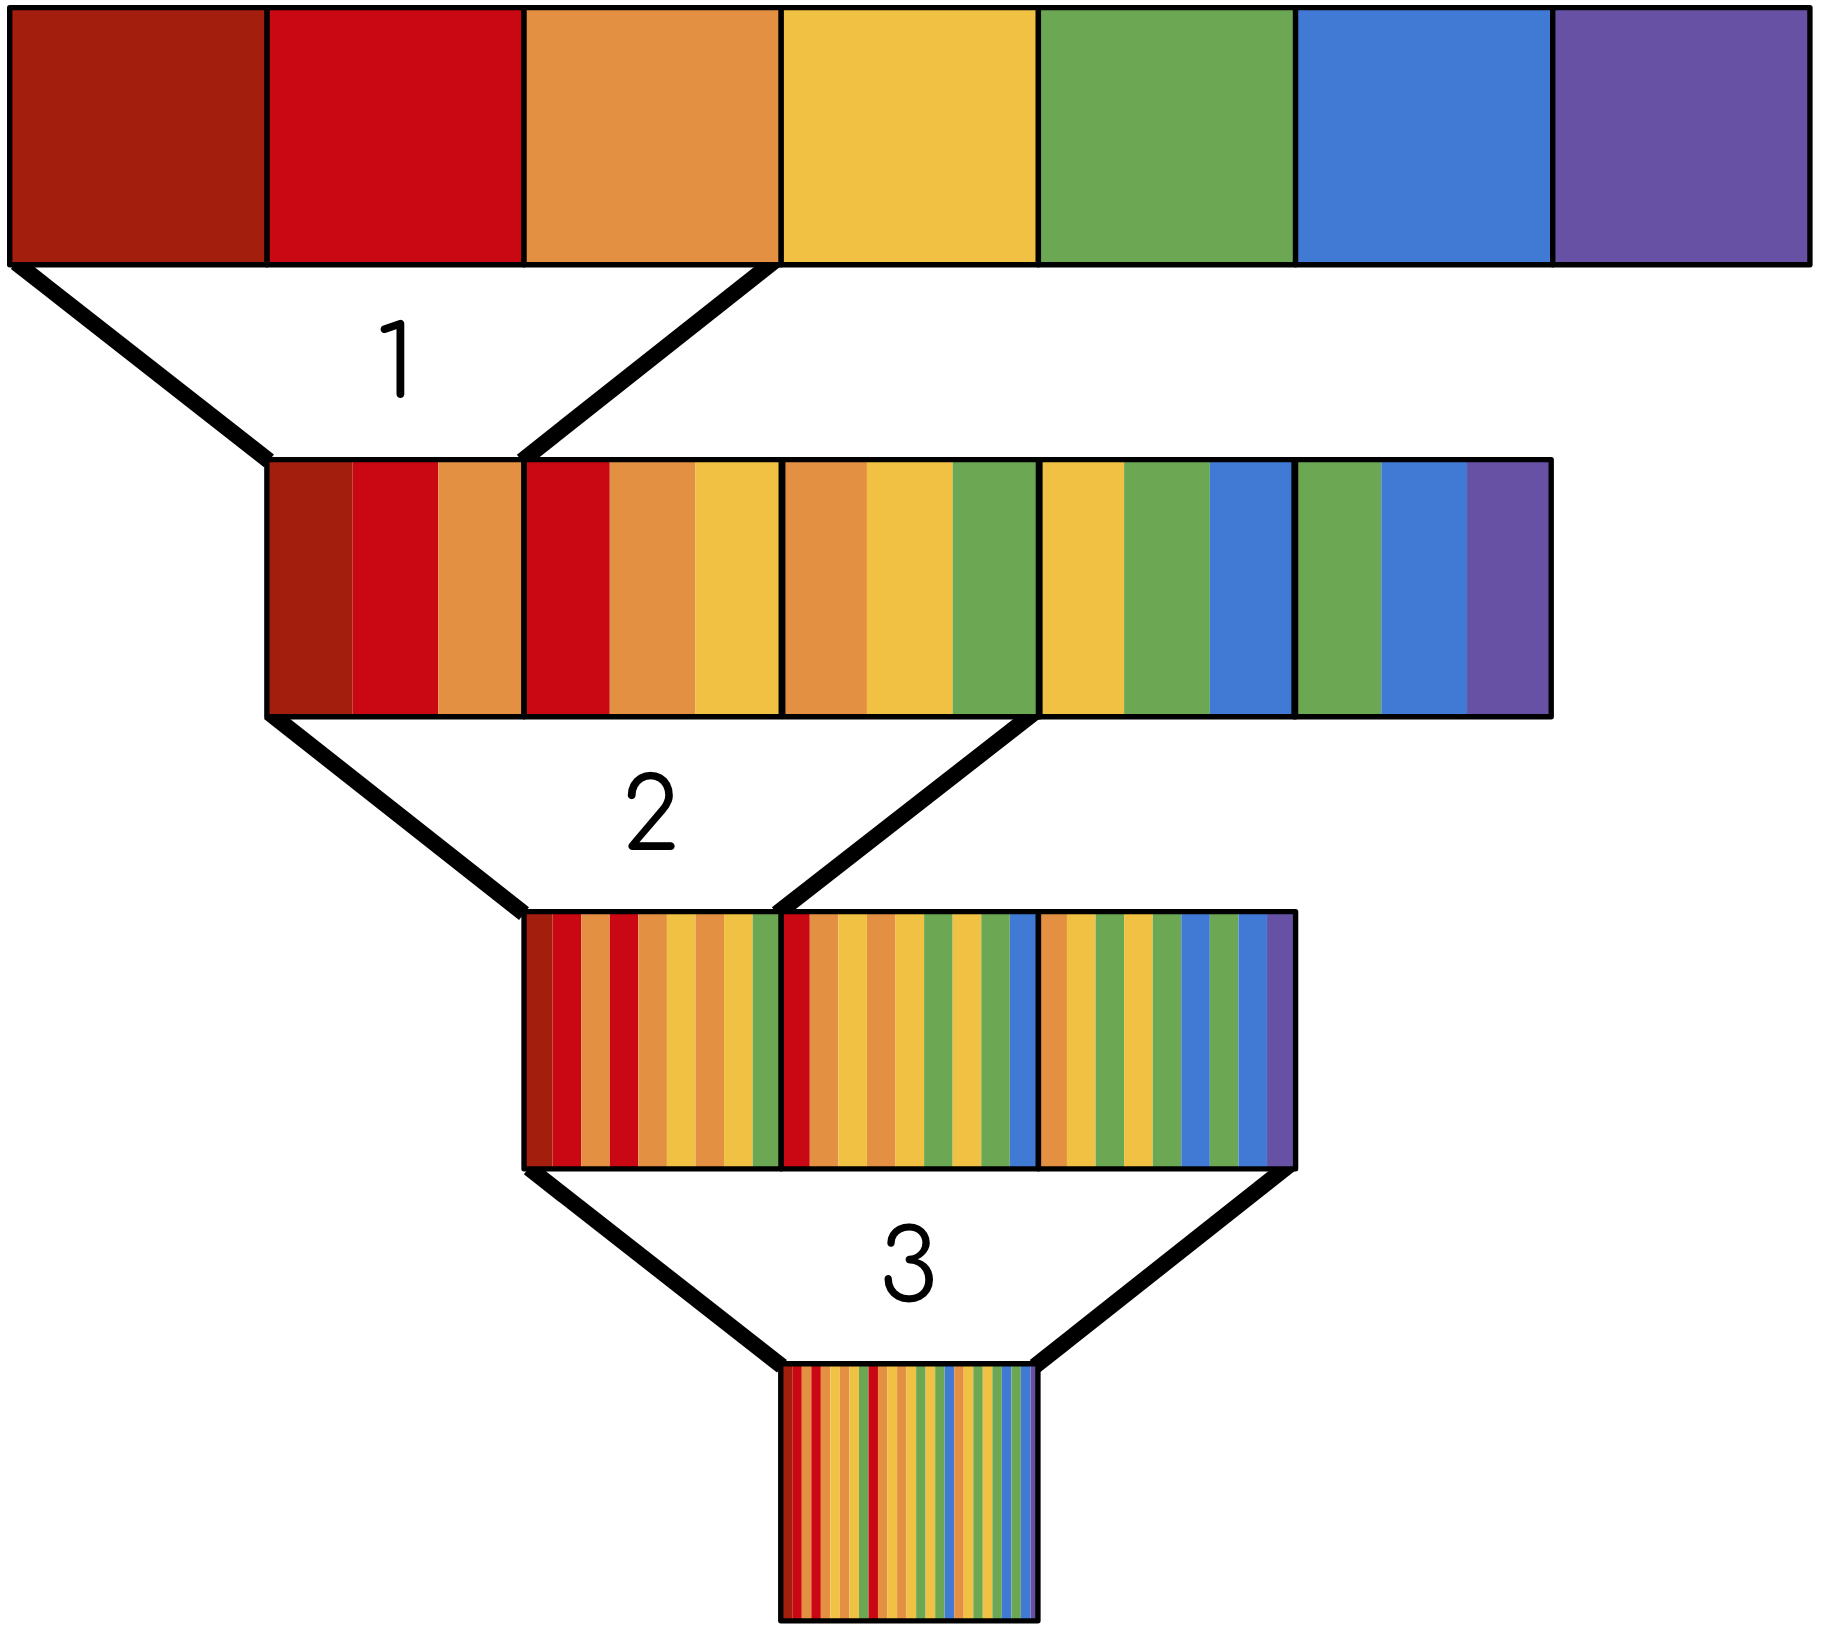
\includegraphics[width=5cm]{receptive}
    \caption[The receptive field of stacked convolutions]{The receptive field of a stack of three 1D convolutions, each with a kernel size of 3 pixels. Notice
    the stacking effect of the convolutions; by the third filter a single pixel contains information (in this example,
        the original color) from all 7 original pixels.}
    \label{fig:receptive}
\end{figure}

The stack of 3x3 kernels requires fewer parameters than the 7x7 case ($3\times(3\times 3)=27$ vs $7\times7=49$)), and nonlinearities
can be placed between each layer of the stack, allowing for much greater flexibility in the functions that can be
approximated by the stack.

The second design choice was to ensure that in each location where the spatial dimensions of the data are halved
through the use of a stride-2 pooling operation, there is a corresponding upscaling of the channels by a factor of 2.
The rationale for this is explained in a later paper by~\cite{he2015}; the computational complexity of the operation
is preserved. The reasoning is thus: halving the spatial dimensions of an image reduces the number of available locations to convolve by a factor of four.
From equation~\ref{eq:conv} (replicated below), the number of computations required to compute a single channel
$C_n^{out}$ of a multichannel convolution scales by factor of $M$:
\begin{align}
	\mathbf{C}^{out}_{n} = \sum_{m=1}^{M} (\mathbf{C}^{in}_{m} \circledast \mathbf{K}_{nm}).
\end{align}

\noindent Therefore, the number of operations to compute $C_n^{out}$ for all $n \in {0, 1, \dots , N}$ scales by $N*M$.
By doubling the input and output channels of the operation, this complexity becomes \newline $2N * 2M = 4NM$,
thus compensating for the 4x reduction of spatial locations. While there is no analysis to motivate this choice
from a model performance perspective in either paper, its conceptual tidiness has caused it to become a widespread
convention in network design.

Using these concepts, \citeauthor{simon2014} present networks of varying scales, the largest being 19 layers deep. They
found that depth was a crucial factor in terms of network performance, with their deepest models performing best. Their
models were evaluated over the ILSVRC ImageNet dataset with a number of training schema, and their best performing
configuration achieved 23.7\% top-1 accuracy and 6.8\% top-5 accuracy.

\subsection{Inception}
Published just two weeks after the VGGNet paper was \hyperlink{cite.szegedy2014}{``Going Deeper With Convolutions''} by~\cite{szegedy2014}.
The paper starts by noting that the deeper-is-better conclusion reached by VGGNet comes with major drawbacks;
exponentially increased computational complexity and increased sensitivity to overfitting. They conclude that to fix
these issues, network design must move from dense connectivity, where every filter is connected to every
subsequent filter, to sparse connectivity. However, due to the relative computational inefficiency of sparse tensor
operations, \citeauthor{szegedy2014} instead attempt to emulate sparse connectivity through dense operations, replacing a single
convolutional layer with a parallel set of 4 operations (1x1 convolutions, 3x3 convolutions, 5x5 convolutions,
and 3x3 max pooling) dubbed the Inception cell, as shown in Figure~\ref{fig:inception}.

\begin{figure}
    \center
    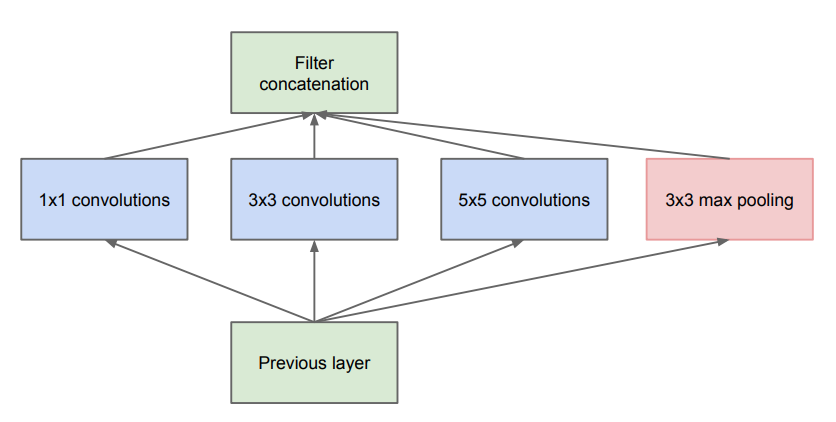
\includegraphics[width=.8\linewidth]{inception_cell}
    \caption[The Inception cell]{The Inception cell as shown in the original paper.}
    \label{fig:inception}
\end{figure}

In the simplest form of the Inception cell, each of the four parallel operations receives an entire copy of the
input information, and outputs a tensor containing a certain fraction of the original channels. This fraction is chosen
such as to weight this operation against the others in the parallel group, and this weighting is varied throughout the network.
The distribution of weights is chosen in accordance with the authors' hypothesis that the data passing through early layers
contains small clusters of local correlation, much like the arguments in~\cite{kriv2009} on data correlation of real images.
These small clusters are then distributed into larger patches later in the network by the
convolutional stacking phenomenon shown in Figure~\ref{fig:receptive}. As such, 1x1 convolutions constitute a large fraction
of the earlier layers of the model, having the smallest kernel size of the available operations. Later layers distribute
the workload more to the operations with larger kernels like the 3x3 and 5x5 convolution.
The output tensors from the four parallel operations are then concatenated together channel-wise, returning a tensor
with the same shape as the original output. This emulates the filters acting over the tensor sparsely, in that only certain parts of the output tensor
have been operated on by any specific filter. The Inception cells are then stacked nine times in the final model,
with pooling layers distributed throughout.

In addition to the novel non-linear architecture of the cell itself, the paper also introduces the concept of auxiliary
classifiers. These arise to solve the vanishing gradient issue through such a deep network; the signal from the loss
function needs to be able to traverse the entirety of the way back up the model in order for every component to
learn effectively. In large networks, this signal often degrades before it can reach the upper layers of the model,
meaning many parameters end up being wasted. To mitigate this, additional classifiers are placed at intermediate points
throughout the model. The predictions outputted by these auxiliary classifiers are passed through the loss function,
and a small fraction of this loss is added to the overall loss of the model. This incentivises the model to find
locations in the loss landscape that produce adequate performance from the auxiliary classifiers in addition
to good performance from the final classifier. Essentially, auxiliary classifiers partition a single model into an
overlapping group of models that each individually need to be effective. Furthermore, the auxiliary classifier introduces
multiple sources of gradient signal all throughout the model, allowing training to happen much more effectively in the
earlier layers of the model. This allows the Inception model to perform well at depths previously unseen in
network design, with around 100 convolutional layers in the final model.

The model is evaluated over the ILSVRC ImageNet subset, and the best single model found a top-5 error rate 10.07\%. Their
best overall score came from an ensemble of seven models, which together achieved a top-5 error rate 6.67\%, which won the
2014 ILSVRC competition. This performance demonstrated that non-linear networks were one potential path\footnote{A
set of branching paths, one might say.} towards to unlocking
higher performance of convolutional neural networks, and furthermore that extremely deep models were now feasible through
the use of auxiliary classifiers.

\subsection{ResNet}
The next year, another network further demonstrated the abilities of non-linear networks, and that was ResNet, published
by~\citeauthor{he2015} The authors open the paper by commenting
on the conclusions drawn from models like Inception and VGGNet, that deeper models tend to be better performing ones.
From this, they ask if more performance can be found by simply making an even deeper model. However, they note the same
vanishing gradient problem as raised by the Inception authors; the gradient signal does not reach the upper layers of the
model. To demonstrate this issue, they set up a thought experiment: imagine a shallow network A that performs well on a
given problem, and a deep network B constructed by adding layers onto A. There exists a learned configuration for network B
such that each added layer reduces to the identity, and thus this configuration would have equivalent performance to network A. However,
despite the existence of such a solution, existing training methods and networks are unable to reach it.

To address this problem, the authors configure the network to explicitly model residual functions, changing the function
modeled by from $F(x)$ to $F(x) + x$. Pairs of stacked convolutional layers are chosen as the granular `function' of the
configuration, used to model some $F(x)$. Inputs are passed into the convolutional group, but are also copied along an
identity connection that circumvents the operations altogether. The output of the convolutional group is then summed into
the identity connection, thus implementing the residual function $F(x) + x$. This configuration is visualized in Figure~\ref{fig:resnet}.

\begin{figure}
    \center
    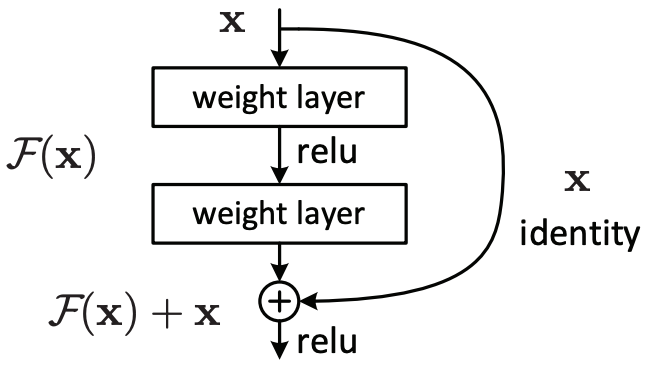
\includegraphics[width=.5\linewidth]{resnet_cell}
    \caption[The ResNet block]{The ResNet block as shown in the original paper. Notice the two discrete paths of the configuration: the
    convolutional operation stack $F(x)$ and the identity $x$.}
    \label{fig:resnet}
\end{figure}

The rationale behind the design decision is that when these blocks are stacked, it creates an unbroken chain of
identity connections that runs the entire length of the model. Gradient signals can thus pass backwards through the model
unhindered and undiluted through the identity operations, while still providing meaningful gradient data through the
convolutions. In addition to this block, a second configuration is designed called the bottleneck block. This block
contains three convolutional layers, the first a 1x1 convolution that reduces channel dimension, second a 3x3 convolution
at these smaller dimensions, and third a 1x1 convolution to return the channel dimension to the original value. These
serve to reduce the parameter size and GPU memory footprint of the models. In the paper, models are constructed that
use the non-bottleneck blocks in 18 and 34 layer configurations, and bottleneck blocks for 50, 101, and 152 layer configurations.
All configurations are then evaluated over the ILSVCR ImageNet subset. If the hypothesis that residual connectivity mitigates
the vanishing gradient problem is true, then the deeper and therefore larger models
should have a greater ability to model the overall problem, and therefore have better performance. To further confirm this,
non-residual models are also evaluated in 18 and 34 layer configurations, identical to the 18 and 34 layers residual models
but with the identity connections removed. In the non-residual configuration, the deeper 34 layer model performed
marginally worse in both train and test accuracy than the 18 layer model, around 0.6--1\% percentage points worse
on both data splits. The opposite was true for the residual configurations; the 18 layer residual model performed
comparably to the 18 layer non-residual model, but the 34 layer residual model scored 3.8\% percentage points better in
test accuracy and around 6\% better in train accuracy. The full results of the 18 and 34 layer comparison are shown in
Table~\ref{tab:resnet1834}:

\begin{table}[ht]
\begin{center}
\begin{tabular}{c|c|c}
                    & Train Error*  & Test Error \\
\hline
18 Layer            & $\mathbf{\approx 31}\%$   & \textbf{27.94}\% \\
34 Layer           &  $\approx 32\%$            & 28.54\% \\
\hline
18 Layer Residual   & $\approx 31\%$            & 27.88\% \\
34 Layer Residual   & $\mathbf{\approx25\%}$    & \textbf{25.03\%} \\
\end{tabular}
\\[1em]
* Train errors estimated by eye from charts in the paper.
\end{center}

\caption[Test and train error of residual and non-residual ResNets]{The test and train error for each of the four configurations in the non-residual/residual
comparison test performed in~\cite{he2015}.}
\label{tab:resnet1834}
\end{table}

These results confirm that the residual blocks do allow for significant improvements in both learning and generalization
performance in deeper models. Much like the results of the Inception paper, it suggests that the additional parameters
of deeper models can be very powerful, if a method can be found to allow for their effective training.
However, upon analysis of these results the authors find that the non-residual models did not suffer from vanishing
gradients despite performing poorly; the batch-normalization layers within the model ensured that there was always
nonzero gradient during backpropagation, and gradient signals were ``healthy'' through the entire model. The authors
speculate that the difficulty in training large non-residual networks is not due to vanishing gradients, but rather
that they just converge very slowly. Whatever the problem may be, it is clear that the residual connections manage to
resolve it.

The three larger bottleneck configurations of 50, 101, and 152 layers show further gains, with performance increasing
monotonically with size up to 19.38\% top-1 error and 4.49\% top-5 error in the 152 layer case. This final model set the
record at the time for the best single model performance on ImageNet, while an ensemble of ResNet-152s also set a record
for the ensemble setting. These results further confirm that the residual block unlocks effective training for very
large models, and that deepening models is a rich vein to mine for better performance.


\section{Neural Architecture Search: First Generation}
\subsection{NAS-RL}
Designing neural architectures is an immensely expensive task, in terms of time, cost, and intuition. Testing a design iteration
can take multiple days of compute time on specialized hardware, and this process can be essentially endless, as the space
of possible architectures is infinite. Furthermore, neural architectures of any meaningful scale are black boxes, which makes
deciding which design change to make and when is a difficult, amorphous problem. That means that there is no guarantee that any
design change made is one in a positive direction, and there is no quick indication that any architecture has reached
the upper bound of possible performance on a problem. These barriers to entry mean that access to state-of-the-art networks
is either granted through incredible luck, or more commonly, immense resources. Those who can afford to throw endless computational
time at a problem can explore more of the search space, experiment with new configurations, push the boundaries, and those that
are unable to cannot utilize the power of deep learning to its fullest. However, the problem of network design is very similar to that of
of feature engineering; an immensely difficult and nebulous task that required a lot of time, experimentation, and intuition.
However, neural networks have managed to almost entirely automate feature engineering away.
The natural question is therefore: can the problem of architecture design be automated too?

While this question had existed for a while, the explosion of GPU-accelerated deep learning in the first half of the 2010s brought
it to the forefront, and a 2016 paper by~\citeauthor{zoph2017} gave its name to the answer:
Neural Architecture Search or NAS\footnote{At the time of original publication of Neural Architecture Search with
Reinforcement Learning, the term ``NAS'' solely referred to the algorithm invented by Zoph and Le. However, as time passed, the term NAS
grew to refer to the entire field of automated neural architecture design, and so henceforth I will refer to Zoph and Le's
algorithm as NAS-RL to avoid confusion.}. \citeauthor{zoph2017}'s paper, fully titled ``Neural Architecture Search with Reinforcement Learning'',
was the first to automatically design an architecture that could compete with the best human designed architectures. Their approach
revolves around condensing information about network design such as filter dimensionality and connectivity into a string
encoding, which can then be passed into a recurrent neural network dubbed the ``controller''. The controller outputs
string encodings, which are then decoded into a ``child network'' that is subsequently trained and evaluated. The performance of this
child network is then mapped back to the RNN controller, forming a reinforcement learning cycle. For each child network evaluated,
the controller gains more information about what constitutes a successful neural architecture for that specific problem. In theory,
this information allows the controller to generate a better formed model on the next cycle, iteratively improving the designed
architecture.

For convolutional networks, NAS-RL designs convolutional layers one at a time, selecting filter height,
width, stride, and total filter number for each. Additionally, the inputs of each layer can be completely specified. Child networks
are trained for 50 epochs, and the validation performance over the last five epochs is used as the reward signal back to the
controller. For CIFAR-10, the best model designed by their controller had 37.4 million parameters and scored $96.35\%$ accuracy
over the validation set, which at the time surpassed the record for human designed architectures of $96.26\%$. However, this best model was the result of
both search space and architecture tuning, while the best entirely autonomously designed model had 7.1 million parameters and
scored only $95.53\%$ accuracy. The full results of this model and all others described later in this chapter are compiled
in Table~\ref{tab:nas_comp_performance}.

However, these
results come with a caveat; they required training of 12,800 architectures across 800 GPUs to achieve. Since each architecture is trained
for 50 epochs, that is 640,000 training epochs total required to run their algorithm. At a relatively conservative estimate of one GPU
minute\footnote{GPU minutes/GPU hours/GPU days/etc are metrics used to normalize the effects of multi-GPU parallelism;
they refer to the total length of time an algorithm would take were it run on a single GPU.} per epoch,
this is 1.21 years of GPU time at minimum necessary to achieve this single result. In a later paper~\citep{zoph_sir2017}
they clarify the runtime, stating they used 800 GPUs for 28 days, which corresponds to 537,600 GPU-hours or just over
61 GPU-years. If the 61.93 years of computation was not enough of a barrier, the cost of this computational time on Microsoft
Azure could run to around \$2,150,400~\citep{AzurePricing} at the time of writing. As such, despite being a highly successful
proof of concept, Zoph and Le's algorithm did not come close to solving the original problem; to make deep learning cheaper, faster,
and more accessible.

\subsection{\added{Neuroevolution-NAS}}
While using reinforcement learning to design neural architectures did produce effective architectures, the need for a
recurrent controller does add significant conceptual complexity to the search process. For example, questions like,
``How do we investigate whether the controller is making sensible design decisions?'', or ``How do we design an optimal
architecture of the controller model?'' arise with no clear answer provided. By turning to a simpler design algorithm
these issues are avoided, and in 2017~\citeauthor{real2017} published ``Large-Scale Evolution of Image Classifiers''\footnote{\added{\cite{real2017}
does not provide any name for their algorithm beyond ``Evolution''. Future papers in the field used the term ``neuroevolution''
to describe the algorithm, however, this could be confused with the widely used neuroevolution genetic algorithm. To disambiguate,
this thesis will use ``Neuroevolution-NAS'' to refer specifically to~\citeauthor{real2017}'s algorithm.}} which used an
evolutionary algorithm to evolve a pool of architectures towards state-of-the-art designs, thus creating the second school
of neural architecture search: evolution. The advantage of evolutionary algorithms is that there is no need for any external
controllers, in that the algorithm runs in an unsupervised, autonomous way. Additionally, the design trends preferred
by the algorithm and the progression of those trends is relatively easier to interpret than is the case with reinforcement learning,
simply by sampling the most favored individuals from the gene pool at any given step of the algorithm.

The crux of~\citeauthor{real2017}'s method is the evolutionary algorithm. They define their population as composed of 1,000 individual
trained architectures, with that model's validation accuracy as their fitness. The operation of the algorithm is performed
in parallel, with each concurrent worker selecting two random models from the population and then sampling their fitness.
The better performing model of the two is selected for `reproduction', which entails cloning the parent model and mutating
the architecture of the cloned child. Both the parent and child are then returned to the population for future selection.
The worse of the two originally selected models is `killed'; i.e, immediately removed from the gene pool.

Also crucial to the design of an evolutionary algorithm is the exact definition of an individual and the specific mechanism
of each individual's reproduction. \citeauthor{real2017} use a directed acyclic graph to represent each individual, with vertices
representing activation functions and edges representing tensor operations. These operations are either identities or
convolutions, with various hyperparameters that control their specific mechanisms of operation. Mutations over these
architectures are then randomly selected from a set of 11 available mutations, which either modify the graph connectivity,
insert operations, adjust the hyperparameters of existing operations, or alter the training dynamics of the model. Within
each mutation there is further random variability; for example, the operation insertion mutation randomly selects
different operation parameters like stride and batch-normalization presence. This means that the true pool of mutations
is multiplicatively larger than 11, providing an immense range of possible options for variation. The
intent of each of these mutations is that they each emulate the design tweaks a human designer might make when trialing
new architectures, such as to constrain the possible mutations into a familiar range.

To determine fitness of any particular individual in the population, \citeauthor{real2017} train each model on CIFAR-10 for
roughly 28 epochs using a fixed learning rate and identical hyperparameters across each run. After training, the model
is evaluated over a held-out validation set of 5,000 examples, and this performance determines the evolutionary fitness
of this candidate. Depending on the size of the individual model, this training process can take anywhere from a few
seconds to a few hours.

Assuming a runtime somewhere in the middle of this range, evaluating the entire population of 1,000 individuals would
take on the order of 40 GPU days. To mitigate this cost, the authors use a technique they call ``weight inheritance''
to minimize training time. For each mutation, they identify the minimum amount of new weights that need to be reset or
created in the child model. In the case of adding a new operation, all other operation weights are preserved. The
same goes with operation modification mutations, only the weights of the modified mutation are reinitialized. This
minimizes the training cost of the new models, as the majority of their weights are shared from their parent models.

The novelty of this algorithm is that it starts from entirely trivial conditions; a population of 1,000 single-layer models
with no convolutions. The authors sought to identify whether a simple evolutionary algorithm could rival the learned
intuition that NAS-RL could provide. To thoroughly explore this question, the authors test their algorithm five times and
compare the performance against a randomly guided evolution. On average, \citeauthor{real2017}'s algorithm found an architecture
with mean CIFAR-10 test accuracy of 94.1\%, and roughly 5.4 million parameters, while the random algorithm's best \
architecture scored only 87.3\%. These performances, while not matching the performance of NAS-RL, do indicate that
evolved models from trivial conditions are indeed at least competitive with the state-of-the-art. However,
the main caveat to all these results is the time cost of the evolutionary
algorithm, reported as a total of 250 hours across 250 parallel workers. This corresponds to a true cost of around seven GPU
years, which while monumentally cheaper than NAS-RL's 61 GPU years is still too expensive for the average user.

\subsection{SMASH}
While NAS-RL and \added{Neuroevolution-NAS} both demonstrated promising results, their main flaw was the prohibitive runtimes
incurred by the training of thousands of candidate architectures. One month after the publication of \citeauthor{real2017}'s
\added{Neuroevolution-NAS} paper,~\citeauthor{brock2017} published ``SMASH: One-Shot Model Architecture Search through HyperNetworks'',
which was one of the first papers to place emphasis on minimizing the expensive candidate model training necessitated
by other contemporaries. To do this, \citeauthor{brock2017} frame the neural architecture search problem as follows:
given a certain candidate pool, the goal of NAS is to discern the best model within. There is no need for the evaluation
of these candidates to entail their comprehensive training or even to produce accurate predictions of their performance,
so long as the evaluation is rank-consistent between predicted performance and true performance. This is to say, a Neural
Architecture Search algorithm only needs to correctly predict performance rank to be effective;
accuracy is entirely unimportant. This is the perspective from which SMASH approaches the neural architecture search
program, seeking to evaluate each candidate's approximate performance by approximating their trained weights.

To do this, they make use of a ``HyperNet'', an external neural network that, when given an architecture encoding as
input, outputs trained weights for that architecture. This process consists of two main components; the architecture
encoding and the weight prediction. To encode architectures of arbitrary convolutional models, \citeauthor{brock2017} define a
``memory-bank'' representation of networks, which conceptualizes an architecture as a series of reads and writes to
discrete memory-banks. For example, each operation within a simple serial architecture would load a tensor from the memory
bank, perform some operation, and then overwrite the memory-bank with the new tensor for use by the next operation. This
model would thus be represented as a series of reads and writes over the same memory-bank within the memory-bank representation.
The advantage of the memory-bank representation is that it lends itself well to a binary encoding. In SMASH, the memory-bank
is encoded as a three dimensional tensor, which is comprised of a variety of adjacency matrices and one-hotted properties
that are stacked and combined to form a single tensor.

This tensor serves as the input to their HyperNet, which takes the encoded architecture as input and outputs a large tensor,
which is then mapped into various architecture weights via a specific slicing scheme based on the layer configuration. The
HyperNet is trained by looping through the following steps a number of times:

\begin{enumerate}[itemsep=-2mm]
    \item Sample random architecture $c$ and data batch $x$.
    \item Pass random architecture through Hypernet $H$ to find output weights $W = H(c)$.
    \item Backpropagate error of $c(x\;|\;W)$ backwards through $c$ and $H$.
\end{enumerate}

\noindent With the Hypernet satisfactorily trained, the weights of any arbitrary number of networks can now be generated rapidly,
which in turn allows for those networks' performances to be ranked. Assuming that the performance ranks from the generated
weights correlates to the true performances of the model, the best model from this sampling can then be trained fully, and
thus the final model is found. To evaluate the validity of the correlation assumption,~\citeauthor{brock2017} train 50 random
CIFAR-100 architectures and compare their true trained validation performance against their SMASH-weighted validation
performance, which is shown in Figure~\ref{fig:smash}. While not perfect, the correlation is remarkably strong, despite
the minimal accuracy of the SMASH-weighted performances.
\begin{figure}
    \center
    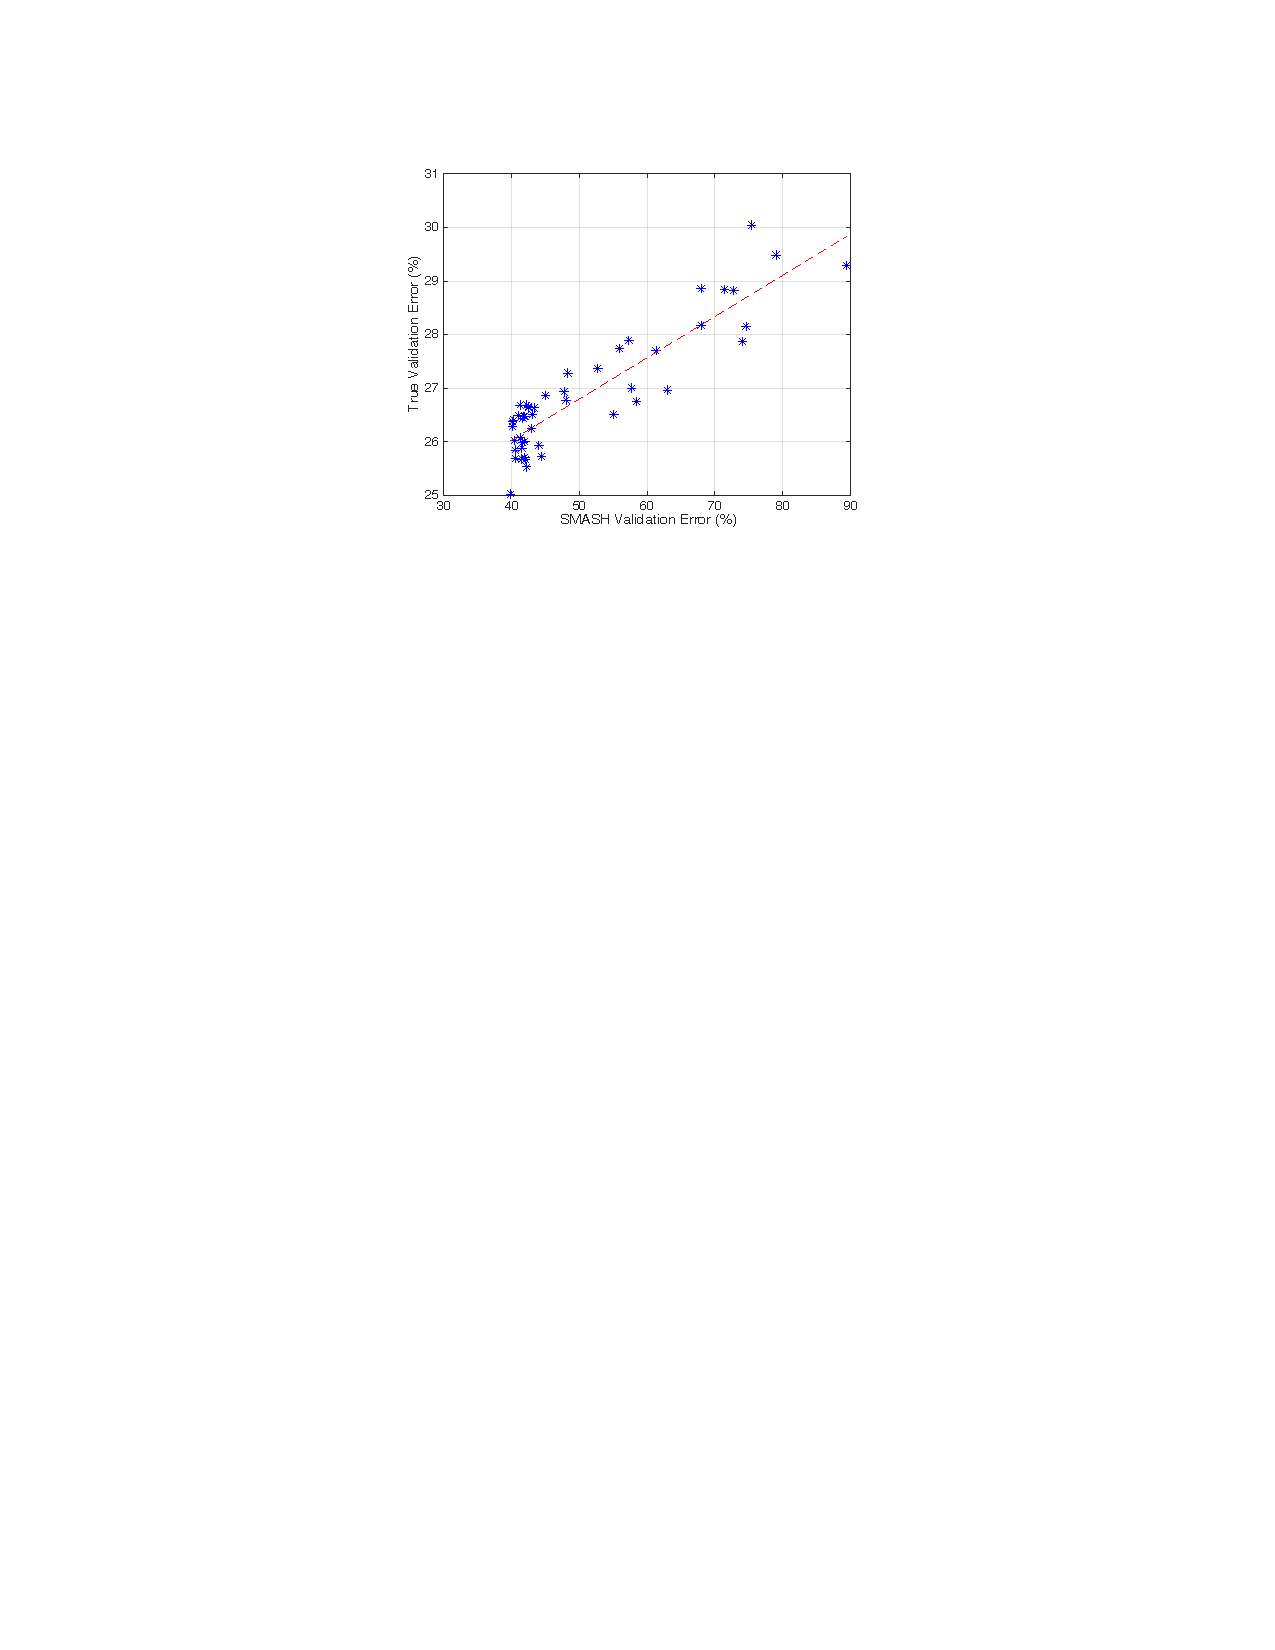
\includegraphics{smash}
    \caption[Correlation of SMASH-weighted models to regular training]{Correlation of SMASH-weighted model performance
    versus their regularly trained performance, as shown in~\cite{brock2017}.}
    \label{fig:smash}
\end{figure}

Another crucial experiment the authors perform to evaluate their algorithm is to test the quality and specialization of
the weights generated by the HyperNet. To do this, they take the input encoded architecture $c$ and perform some corruption
of the encoding, generating a new encoding $c'$. The weights generated by the HyperNet $W=H(c')$ are then used to set the
weights of original architecture $c$. This means that the HyperNet ``thinks'' it is generating weights for an architecture
$c'$, but is actually generating weights for $c$. If there are no meaningful performance differences between $c$ and $c'$
over a variety of corruptions, the mapping learned by $H$ is not truly learning to tailor weights to specific architectures,
but is rather a favorable general case that always produces decent results. However, the authors find that the best performance
is consistently found when $c=c'$, that is, when the model's expectation of the architecture it is being asked
to generate weights for matches the actual architecture used. This implies the model does take into account the architecture
at hand, and is producing specialized weightings.

With the methodology validated, \citeauthor{brock2017} report the performance of SMASH. They report two different CIFAR-10
performances, corresponding to two different HyperNet configurations and search space parameters. The first, named SMASHv1,
achieves a 94.47\% test accuracy with 4.6 million parameters, while the second scores 95.97\% accuracy with 16 million parameters.
While these results are again surpassed by those of NAS-RL, the runtime of SMASH is the standout advantage. While not directly
reported in the paper, other sources have reported the runtime to be around 1.5 GPU days~\citep{ren2020}, which makes sense;
not needing to fully train thousands of candidate architectures should drastically reduce the time costs.
Furthermore, the entire algorithm runs on a single GPU, which significantly lowers the hardware costs and overhead compared
to the massively parallel setups seen in competing algorithms. This is the first algorithm to demonstrate that competitive
results can be attained on the order of days, not months or years, thus setting a very high bar for search efficiency.

\subsection{PNAS}
One final contribution to the first generation of neural architecture search algorithms is~\citeauthor{liu2017}'s 2017 paper,
\hyperlink{cite.liu2017}{``Progressive Neural Architecture Search''}, which notes the immense cost of~\citeauthor{zoph2017}'s NAS-RL and~\citeauthor{real2017}'s
\added{Neuroevolution-NAS}. They argue that the need to train thousands of candidate models is not only overly wasteful
in time cost, but also simply an inefficient means of traversing the search space. To remedy this, they introduce
a ``progressive'' means of traversing the search space of available models from most simple to most complex. This entails
dividing the construction of each possible model into its component building blocks, with the simplest models
comprising of just a single block while more complex models are comprised of many blocks connected in more complex patterns.
From this search space, the set of the simplest models is identified, i.e, the ones that only require a single block.
This is a tiny subset of the full search space, and it is relatively easy to fully train each of them in parallel.
Each of these simplest models is then expanded upon, by looking at the models that can be created by adding a single
extra block to the existing configuration. This rapidly expands the space (there are around 147,000 candidate models after
only two blocks), which makes fully training each of the candidate models untenable. To circumvent this issue,
\citeauthor{liu2017} apply a learned predictor, which seeks to predict the performance of a model given its block structures. This
predictor takes the form of a recurrent neural network, that takes the model configuration encoded in string-form as its
input much like~\cite{zoph2017}. From the set of expanded models, the predictor selects the $K$ most promising, where
$K$ is chosen such that $K$ models are quick and practical to fully evaluate in parallel. This process continues until
a sufficiently complex and performant model is discovered. This found model is then fully trained according to a fixed
set of hyperparameters.

In essence, PNAS performs a depth-first search of the search space; eliminating entire branches of the search tree if
they are not favorably viewed by the predictor and instead traversing downwards towards promising leaves. From this heirarchical
search tree perspective algorithms like NAS-RL and \added{Neuroevolution-NAS} appear starkly inefficient; their traversal
of the search space does not take advantage of the structures of the space that can be exploited in the name of optimization.
To elucidate the advantage provided by the heirachical search, \citeauthor{liu2017} compare the total number of model trainings
necessary between their algorithm and that of NAS-RL, and they find their algorithm requires 1.8 times fewer
trainings then NAS-RL to find competitive architectures, despite traversing an identically sized search space.

\citeauthor{liu2017} run the PNAS process five times over a variety of search space and model parameters, and report the CIFAR-10
results of the five models identified, each of which are trained 15 times with different random seeds and initializations.
The best model, titled PNASNet-5, achieved a mean test accuracy of 96.59\% with 3.2M parameters. However, these results
share a similar caveat to those seen earlier, which is in their hardware and runtime requirements. Crucial to the PNAS
algorithm is the parallel evaluation of around 1,200 models, which requires either an immense number of GPUs or
a very large runtime. While the exact runtime of their algorithm is not reported, they do claim a 15$\times$ speedup
compared to NAS-RL, which would imply a runtime of around 2,500 GPU-hours. Again, despite excellent performance,
the algorithm is out of reach to the average user.

\section{Neural Architecture Search: Second Generation}
With algorithms like NAS-RL, \added{Neuroevolution-NAS}, and PNAS demonstrating that automated network design was indeed possible, and the
results of SMASH showing that efficient search can happen on the order of days, not months or years, the first generation of neural
architecture search demonstrated the promise of the field in both raw performance and efficiency. However, no algorithm had
succeeded in both dimensions to any significant degree, which left the door open for a new class of algorithms that could
achieve state-of-the-art results in minimal runtimes. To fill this hole came the second generation of neural architecture
search algorithms, which all sought to update and optimize existing algorithms or pioneer entirely new ways of
mitigating the faults of the prior generation.

\subsection{NASNet}
First of the second generation of NAS is \citeauthor{zoph_sir2017}'s 2017 paper \hyperlink{cite.zoph_sir2017}{``Learning Transferable Architectures for Scalable
Image Recognition''}. This builds upon their earlier results of NAS-RL via search space tailoring,
through two specific decisions. First, they adapt a cellular design pattern for their models.
This is reminiscent of the block concept of models like ResNet and Inception, where a local connectivity pattern (a cell) is
designed and then stacked at varying scales to produce a final network. This modularity lends itself to significant flexibility
in terms of the final network architecture, the topography and total size of the
network can be altered just by changing the number or position of cells. Here, two cells are designed for
each final convolutional architecture; a ``reduction'' cell and a ``convolution'' cell. In reduction cells, the channel dimensionality
of each tensor that passes through the cell is doubled, while the spatial dimensions are halved. Convolution cells do not modify
tensor dimensionality in any way. The cellular design philosophy dramatically reduces the search space size, as the
algorithm only needs to design two cells rather than a full model. In the specific case of this paper, there are
either 14 or 20 cells in a full CIFAR-10 model, thus reducing the size of searched model by a factor of 7 or 10,
respectively. Furthermore, \citeauthor{zoph_sir2017} note that an algorithm that returns modular cells is more generalizable than
an algorithm that produces a monolithic architecture, in that these cells can be stacked in novel ways and at various channel dimensions
to suit different tasks. In \citeauthor{zoph_sir2017}'s experiments, they choose two reduction cells for CIFAR-10, stack $N$ normal cells before each reduction cell,
and place an additional $N$ normal cells after the final reduction cell.

Second,~\citeauthor{zoph_sir2017} limit the search space down to a fixed set of 13 operations\footnote{The 13 operations are: Identity, $1\times3$
    and $1\times7$ rectangular convolutions, $3\times3$, $5\times5$, and $7\times7$ max poolings, $3\times3$ average poolings,
    $1\times1$ and $3\times3$ convolutions, and $3\times3$, $5\times5$, and $7\times7$ depthwise-separable convolutions.}
and connectivity patterns. Each cell receives the output of the two previous cell $h_i$ and $h_{i-1}$ which are dubbed the first two
hidden states, and constructs cells as follows:

\begin{enumerate}[itemsep=-2mm]
    \item Select two hidden states from $h_i$, $h_{i-1}$, or from the hidden states created in earlier iterations.
    \item Select two operations to apply to the first and second chosen hidden states, respectively.
    \item Select either element-wise addition or concatenation to combine the two operation outputs.
    \item Add the combined outputs to the available hidden states.
\end{enumerate}

\noindent By repeating these steps a certain number of times, cells of varying sizes and connectivities can be constructed.
In their experiments, \citeauthor{zoph_sir2017} settle on five iterations to produce consistently good results, therefore producing cells
with around 10 operations each.

This design pattern, specifically the fixed operation set, cellular design pattern, and specific connectivity pattern, is
codified as the NASNet search space, to provide a consistent baseline comparison between architectural search techniques.
This is important such as to differentiate between the improvements brought by better search spaces versus better
architecture search methods, as both dimensions can produce meaningful impact on results and thus must be disentangled.

After introducing the NASNet search space, \citeauthor{zoph_sir2017} run their earlier NAS-RL algorithm within it. They test a variety
of different configurations, but just the best performing run and the most efficient run will be focused on here. The latter
named NASNet-A uses $N=7$, has 576 channels in the first layer of the network, and scores a 97.60\% accuracy on CIFAR-10
with 27.6 million parameters. The former, NASNet-B, uses $N=4$, has 288 channels in the first layer, and scores a 96.27\%
with 2.6 million parameters. While these results are very impressive, the very high runtime cost tempers their real-world
applicability. \citeauthor{zoph_sir2017} actually erroneously report their runtime cost in the paper, stating that their algorithm uses
500 GPUs for four days and thus costs 2,000 GPU-hours to run. This is of course a unit error, as they are reporting their
GPU-\textit{day} cost, not the correct figure of 48,000 GPU-\textit{hours}. This is around 5.4 years, still massively outside the scope
of any average user.

\subsection{ENAS}
In early~\citeyear{pham2018}, Zoph and Le, along with Hieu Pham, Melody Guam, and Jeff Dean sought to address
the criticisms of NAS-RL by releasing \hyperlink{cite.pham2018}{``Efficient Neural Architecture Search via Parameter Sharing''}, dubbed ENAS.
They note that the main inefficiency of NAS-RL was the requisite training of each child network produced by the controller.
To remedy this, they introduce the concept of a weight-shared supernet. The idea is that instead of creating thousands of
independent child networks, one should instead create a single massive ``supernet'' such that every possible child network is a subgraph of the parent graph.
The supernet as a whole is then trained for a single epoch over the training data. From this point onward, the general concept
of the ENAS algorithm is roughly similar to that of NAS-RL; an RNN controller designs neural architectures layer-by-layer,
iteratively selecting the parameters of the layer. However, once the architecture embedding is generated by the controller
it is instead extracted from the supernet and evaluated over a held-out validation set. The performance on the validation set
is then passed back to the controller as a reward. Before generating the next architecture, the supernet is trained for another
epoch. These training phases between the supernet and the controller continue to alternate throughout the whole process, until a
final architecture is selected. In essence, at any particular training epoch the supernet seeks to model the weights of
any particular subnetwork after an equivalent number of epochs, while the controller attempts to identify the most promising
subnetwork within the supernetwork at that point in time, with the hope that both will iteratively improve in performance
over time. Since there are only two networks to train, the supernetwork and the RNN controller, the whole process can be up to
50,000 times faster than NAS-RL.

The second key concept to the ENAS paper was that of the micro-search space. While ENAS is capable of designing an entire network
from the ground up (dubbed the macro-search space in the paper), it is also able to work on a cellular basis, instead designing
convolutional and reduction cells that are then stacked according to a predetermined pattern:
21 total cells with reduction cells in positions 7, 14, and 21 and convolution cells in the rest. In the macro-search space over
CIFAR-10, ENAS was asked to design 12 layer networks, the best of which had 38.0 million parameters and scored
an accuracy of 96.13$\%$ over the CIFAR-10 test set. In the micro-search space, ENAS produced a model with 4.6 million parameters
that scored an accuracy of 97.11$\%$.

However, the most important result from ENAS was not its raw performance, but rather the relatively small amount of
time and resources necessary to achieve those results: ENAS takes only 16 hours and a single NVidia 1080Ti GPU to run.
A GPU of similar performance can be accessed on the cloud for around \pounds1-\pounds2 an hour~\citep{AzurePricing}, meaning that
ENAS entirely remedies the prohibitive costs and runtime of NAS-RL. The sub-1 GPU day benchmark set by ENAS remains an
important goal in the field of NAS to this day, with authors constantly competing to further lower the
computational cost of NAS~\citep{liu2018,xu2020}.

The cost dichotomy between NAS-RL and ENAS represents two possible directions for the field of NAS. The former looks to
discover the best possible networks regardless of computational cost, looking to throw functionally infinite resources at the
problem to discover the absolute limits of performance~\citep{pham2018,huang2018}. The second looks to minimize
the temporal, fiscal, and computational outlay of NAS, to bring it as close to the average user as possible. The latter
direction is one that seems more magnanimously valuable to pursue; not only is achieving competitive results in the most
efficient way possible an intellectually interesting problem, it is also one with a much broader accessibility.
There are very few entities out there that could justify the outlay that an algorithm like NAS-RL requires simply to
produce a single neural architecture, but almost everyone with access to a GPU could run something like ENAS.

\subsection{Regularized Evolution}
Contemporaneously to ENAS, \citeauthor{real2018} published \hyperlink{cite.real2018}{``Regularized Evolution for Image Classifier Search''},
which sought to improve upon their earlier \added{Neuroevolution-NAS} paper. Here, \citeauthor{real2018} note the relatively poor performance
of evolved models compared to the state-of-the-art hand-designed ones, and attempt to improve their evolutionary
algorithm in the hopes of facilitating the discovery of higher-performing models.

The first difference introduced by their new algorithm comes down to how models are removed from the population; previously,
the worse-performing model of the two selected in the random-tournament was discarded. Now, the age of each model
in the population is tracked, and the oldest model is removed. In practice, this means that the model that was trained
the earliest is removed from the population every time a new model is introduced. To explain the advantage of this approach,
\citeauthor{real2018} compare their old, non-aging evolution to aging evolution. Specifically, they introduce the concept of a
lucky model, one that arrives at an unreproducibly high accuracy early in the algorithm simply by random chance and
might not actually perform all that well when retrained. In non-aging
evolution, this result will be maintained as a promising path for evolution and as such will spawn many offspring as
the algorithm attempts to refine the architecture. However, since the architecture simply scored well due to lucky
training, all the children will likely perform worse and thus be wasted search time. This problem will continue until
the lucky model is removed from the search space, which will only happen when it is compared against a better model, which
can only occur if the algorithm has identified such a model. However, the presence of a lucky model in the population
will reduce the chance of the algorithm ever identifying a better model, as exploring the children of the lucky model
distracts the algorithm from better options.

If such a lucky model is placed into an aging algorithm, it can only remain in the search space for a short period before
it ages out of the population. This means that the time wasted exploring its children is limited, and unless it can produce
good offspring its architectural genetics will not be preserved. This leads us to the main crux of aging evolution:
architectures can only last in the population if they produce consistently good descendants, thus biasing the algorithm
towards architectures that are repeatedly well-performing and are fruitful candidates for evolution.

The second key change introduced is to align the search space to the NASNet search space, by ensuring that all initial
members of the population conform to the NASNet specifications and that mutations only produce similarly compliant models.
This allows for direct comparison against other NASNet-conforming algorithms. \citeauthor{real2018} call the models produced by
their algorithm AmoebaNet, and their best model over CIFAR-10 scored a 96.66\% accuracy with 2.6M parameters. However,
it exacerbates the runtime problems of \added{Neuroevolution-NAS}, in that it requires 450 GPUs over seven days, a total of 75,600
GPU-hours or 8.63 GPU-years. This is around a year and a half more expensive than \added{Neuroevolution-NAS}, and it is still entirely
unfeasible for the average user to reproduce their results.

\section{Differentiable Architecture Search}
\subsection{DARTS}
Despite ENAS' accessibility, it has an implicit inefficiency in the need to jointly train the supernet and the recurrent
controller. If the supernet contains all possible architectures, the controller serves only as a means of identifying
the most promising subgraph. This is to say; training the supernet already produces the result, it just needs to be
isolated in some way. Identifying a way to train the supernet whilst whittling it down to some optimal subgraph
would complete architecture search without need for external controllers. This is exactly the reasoning behind \citeauthor{liu2018}'s
2019 paper \hyperlink{cite.liu2018}{``DARTS: Differentiable Architecture Search''}.

DARTS compartmentalizes architectures in a similar way to ENAS, in that it searches for a small, modular neural cell
that it can stack into larger networks. These cells are explicitly graph structured in the paper, where nodes represent
locations in the model where tensors are combined, such as through concatenation or summation. Edges represent
operations over tensors, such as convolutions or pooling operations. Sample neural cells depicted in this
graph structure are shown in Figure~\ref{fig:darts}.

\begin{figure}
    \center
    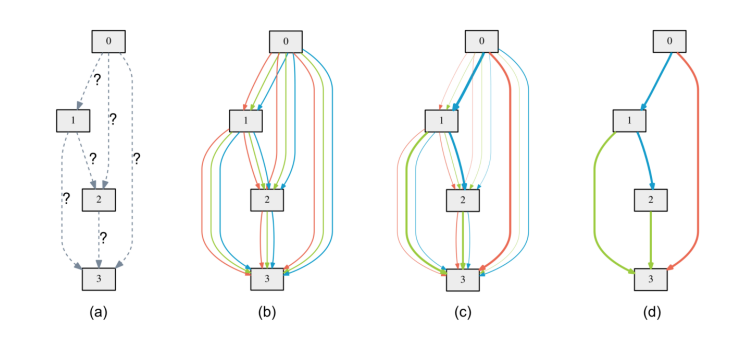
\includegraphics{DARTS_cell}
    \caption[DARTS' graph representation]{The graph representation used by DARTS as it appears in the paper. Data flows from top to bottom, nodes are
    tensor combinations, and edges are transformations.}
    \label{fig:darts}
\end{figure}

While there a number of ways to represent architectures via graph (such as the Inception paper, which represents both
operations and combinations via nodes and instead uses edges to show data flow), the DARTS abstraction
can be exceptionally helpful in conceptualizing the connectivity of nonlinear architectures. From this point onwards all neural
architectures will be represented according to the DARTS graph representation unless otherwise specified.

To design a cell, DARTS first needs a set of candidate operations $\mathcal{O}$ and a number of nodes per cell $N$.
These $N$ nodes are then placed into the graph, and numbered sequentially from 0 to N.
Then a set of $|\mathcal{O}|$ edges, one per operation in the search space, are placed between each pair of nodes n and m
such that $m>n$. This means that each node has outbound edges to every subsequently numbered node, but not to antecedent
nodes. Figure~\ref{fig:darts}b shows this configuration n the case where $N=4$ and $|\mathcal{O}|=4$.
This configuration forms the DARTS supernet,
where every possible cell containing $N$ nodes and $|\mathcal{O}|$ available operations appears as a subgraph.

The key to whittling this supernet down to the final architecture is translating the discrete choice of operation between
each edge into a continuous one. This is accomplished by assigning a weight vector $\mathbf{\alpha}_o$ of size $|\mathcal{O}|$
to each set of parallel edges. The weight vector is softmaxed and used to perform a weight sum of the parallel edges. This
transforms a set of parallel operations $(o_0^{(i,j)}, \;o_1^{(i,j)}, \quad\dots\quad, o_{|\mathcal{O}|}^{(i,j)})$ into a single
operation $\bar{o}^{(i,j)}$, a continuous mixture of the entire set:
\begin{align}
    \bar{o}^{(i,j)}(x) &= \sum_{o \in \mathcal{O}} \frac{\exp\alpha_o^{(i,j)}}{\sum_{o \in \mathcal{O}}\exp\alpha_o^{(i,j)}} \; o(x). \label{eq:darts_ops}
\end{align}

By making the weight vector $\mathbf{\alpha}$ a differentiable parameter of the supernet, it can be learned
via gradient descent; meaning that the architecture of the model is now itself learnable and optimizable. This therefore
removes the need for an external controller entirely, with the possibility for combining architecture selection seamlessly
with model training. However, Liu, Simonyan, and Yang choose to keep the two processes separate, this decision motivated
by structuring the architecture weights and network weights as separate variables in a bilevel optimization problem.
They approximate a first-order and second-order solution to this optimization problem that differ slightly in terms of
their formulation, accuracy, and requisite computational complexity, but both consist of alternating between
updating architecture weights and network weights, keeping one fixed whilst learning the other.

After the architecture weights and network weights have converged sufficiently, a discrete architecture is extracted by
selecting the operations with the highest nonzero weights, such that only one operation per parallel operation set is
selected. This discrete architecture is then retrained from scratch. On CIFAR-10, first-order DARTS discovered a 3.3 million
parameter model that scored a test accuracy of $97.00\pm0.14\%$, taking 1.5 GPU days to complete the search. Second-order
DARTS found a 3.3 million parameter model with an accuracy of $97.24\pm0.09\%$, but took four GPU days to run.

\subsection{NAO}
The DARTS method of operation mixing is not the only way to produce a continuous search space. Shortly after the
publication of DARTS, \citeauthor{luo2019} published \hyperlink{cite.luo2019}{``Neural Architecture
Optimization''} (NAO) which used an architectural embedding space to produce a continuous search space.
NAO involves three chief components, the encoder, the performance predictor, and the decoder. The encoder is a small recurrent neural
network whose task is to translate architectural configurations, represented via string, into an n-dimensional embedding
space. The performance predictor then maps points in the embedding space into predicted test set accuracy, taking the form
of a single layer feedforward network. Finally, the decoder is another small recurrent neural network which maps embedding
vectors back to architectural representations. These three components are trained jointly with a combined loss function.
Once the three components are fully converged, better architectures can be derived by performing gradient descent over
the embedding space. This entails sampling an architecture, mapping it into the embedding space via the encoder, then
taking a step in the most negative gradient direction as determined by the performance predictor. The location of this step
is then passed to the decoder, in theory producing a slightly better architecture than the first. This process is repeated
until the gradient descent converges to a minima, ideally the optimal architecture within the space.

The main downside to the algorithm as presented thus far is that in order to meaningfully learn a mapping between
the embedding space and performance, the performance predictor requires a significant sample of fully-evaluated architectures.
For CIFAR-10, 1000 full architecture evaluations were necessary to achieve convergence, a process that took 200 GPU days to complete.
To mitigate this immense computational cost, \citeauthor{luo2019} adapt NAO to the weight sharing system used in ENAS, where the encoder,
performance predictor, and decoder operate over subgraphs of a supernet. This reduces the necessary architectural evaluations
from 1,000 down to just one, that of the supernet, and reduces the runtime to just seven GPU hours.

For CIFAR-10, the best architecture found by NAO sans weight sharing had 144.6 million parameters,
scored a $98.07\%$ test accuracy, and took 200 GPU days to discover. The best architecture found by NAO with weight sharing
had 2.5 million parameters, scored a $97.07\%$ test accuracy, and took just seven GPU hours to discover.

\subsection{ProxylessNAS}
One potential limitation to the cellular approach used by algorithms like DARTS and ENAS is the assumption that the best
normal and reduction cells will stack to become the best $N$ celled model. However, this limitation is often necessary
as the full supernet for an $N$ cell model would have a intractably large VRAM footprint, whereas a single cell is much
easier to fit onto the GPU. In the 2018 paper
\hyperlink{cite.cai2018}{``ProxylessNAS: Direct Neural Architecture Search on Target Task and Hardware''}, \citeauthor{cai2018}
propose a method to avoid this restriction altogether. \citeauthor{cai2018}'s algorithm is structured very similarly to DARTS,
where a supernet is constructed with each possible operation placed in parallel along the edges. These parallel operations
are weighted via $\alpha_o$ much like DARTS, with the crucial difference lying in the parallel edge computation equation.
Rather than using a softmax summation of each operation as per DARTS (Equation~\ref{eq:darts_ops}),
each parallel edge is computed as follows:

\begin{align}
    \bar{o}^{(i,j)}(x) &=
        \begin{cases}
            o_0(x), &  \text{with probability } a_{o_0}^{i,j} \\
            \dots\\
            o_n(x), &  \text{with probability } a_{o_n}^{i,j}
        \end{cases}~\label{eq:proxyless}
\end{align}

\noindent The selection of operations is one-hot, in that a single operation is chosen at a time. The edge's
operation weights $a_o^[i,j]$ therefore determine how frequently each operation is chosen to be the sole operation
of the edge. This is the crucial difference to DARTS, and drastically reduces the VRAM requirements of the ProxylessNAS
supernet. This is because only $\frac{1}{\lvert \mathcal{O} \rvert}$th of the candidate operations need to exist on the
VRAM at any given time, signficantly reducing the amount of tensor allocations required by the model. This allows the
ProxylessNAS supernet to exist in its complete form directly from initialization, meaning that the entire model
can be directly searched for, rather than single cells as per DARTS.

The difficulty with this approach is that in order to effectively learn the edge weights, the gradient of each weight
must be computed, which in turn is only possible by performing a forward pass through each operation. This would invalidate
the VRAM benefits of the edge one-hotting, and therefore \citeauthor{cai2018} devise a means around this problem. Rather than
learn the entirety of the edge weights at once, they instead formulate it as a tournament selection problem. Their reasoning
for this is that if a particular operation is the best among all the candidates, it should also be the best in the pairwise
comparisons performed in tournament selection. In practice, training of the model happens in two stages. First, the edge
weights are held fixed, and the operations are chosen stochastically as per Equation~\ref{eq:proxyless} and trained normally.
Next, the operation parameters are held fixed, and two operations per edge are selected at random according to the
edge weights. The two corresponding edge weights are updated while holding the other $|\mathcal{O}|-2$ fixed, and as such
only $\frac{2}{\lvert \mathcal{O} \rvert}$ths of the operations need to be held in VRAM, which largely
mitigates the cost of training edge weights.

One potential difficulty with this approach is ensuring that all candidate operations in each edge are trained adequately,
such that they can be compared fairly against the other candidates. Since the edge selection is binary, $|\mathcal{O}|-1$
operations per edge are not trained during each operation training step. If an operation happens to be chosen less frequently
than its competing edge-mates, it will receive less training. Even if this operation would end up being the best of the
candidates after convergence, the fewer training cycles will likely cause it to perform worse than the competition. This in turn
would cause it to be chosen even less frequently, furthering this cycle. However, this can likely be mitigated by
careful choice of the rate of edge weight training, such as not to lock in any decisions prematurely.

After training the edge weights and operation parameters, the final architecture is chosen by selecting the operations
with the highest weights from each edge. This subarchitecture is then trained from scratch. For CIFAR-10, ProxylessNAS
discovers a network that achieves 97.92\% accuracy with 5.7 million parameters. The time cost for the search is not reported in the
paper or in any subsequent papers, but from the details provided in the paper it can be inferred to be somewhere on the
order of a few GPU-days.

\subsection{PC-DARTS}
While DARTS was shown to be effective at finding state-of-the-art architectures, the supernet search method does require
a significant amount of VRAM space to evaluate candidacy of operations that are eventually excluded from the model. This
means that the models are size limited by how big the candidate supernet cell can be. One approach to remedy this
issue is \citeauthor{cai2018}'s edge binarization, but another approach is introduced by~\citeauthor{xu2020}'s 2020 paper
\hyperlink{cite.xu2020}{``Partially Connected DARTS''}~ or PC-DARTS. Here, for each parallel edge of candidate
operation, only a proportion $\frac{1}{K}$ of the input channels to the edge are selected per forwards pass.
This subset passes through the parallel operations, while the remaining channels pass through transparently.
This is highly similar to dropout, with the difference being dropout omits the operation while PC-DARTs replaces it with the
identity. This reduces the computation necessary for each candidate operation significantly as well as reduces the amount
of space each operation needs to allocate by $K$, allowing the use of larger batch sizes or larger models.

The authors note that this channel sampling acts to reduce operational selection bias. They observe that DARTS often
shows bias towards weight-free operations like poolings, as in early stages of the model's lifetime those operations
do not have randomly initialized weights and are thus more reliable. Channel sampling can help this as it reduces
the mathematical difference
between any two operations; $\frac{1}{K}$ of an edge's output channels are operation outputs, while the
other $\frac{K-1}{K}$ are simply identities. Therefore, the choice between one operation versus another affects only
these $\frac{1}{K}$ channels, reducing the possible difference between any two
operations and thus reducing selection bias. The downside to this channel sampling approach is that it implicitly lowers the accuracy of the architectural decisions,
as operations are selected based on their performance over small subsets of the input data. This is unstable, as the
particular subsets that this evaluation is made over are continuously fluctuating. To mitigate this, they introduce
edge normalization, which introduces a set of edge weights $\beta$, such that the computation of a single edge
$i\rightarrow j$ is:
\begin{align}
    f_{i \rightarrow j}(x) &= \frac{\exp \beta_{(i,j)}}{\sum_{i < j}\exp\beta_{(i,j)}} \sum_{o \in \mathcal{O}} \frac{\exp\alpha_o^{(i,j)}}{\sum_{o \in \mathcal{O}}\exp\alpha_o^{(i,j)}} \; o(x).
\end{align}

This adds a second weighting to the configuration; $\alpha$ selects which operations lie along each edge just as in
DARTS, while $\beta$ describes the weight of each edge in the cell. The final architectural decisions are then
chosen as the product of an operation's $\alpha$ weight with its edge's $\beta$ weight. Therefore, operations that
 perform abnormally well for a particular channel subset might get a beneficial bump in their $\alpha$ weight, but it will
be normalized via their overall edge weighting which is invariant to channel sampling.

To compare the additions of partial connectivity and edge normalization, the authors perform an ablation study against
regular DARTS over CIFAR-10. In their experiments, regular DARTS scored 97\% test accuracy. The addition of just
edge normalization increases this to 97.18\%, while just partial connectivity increases it to 97.33\%. Both together
produce the best result, a 97.43\%. However, as the paper's reviewers note, the amount to which these increases are due
to actual search improvements or simply the increased model and batch size afforded by the channel sampling approach is
unclear.

%\section{Other Neural Architecture Search Familes}
%So far a wide variety of schools of neural architecture search have been explored: reinforcement learning
%approaches such as NAS-RL or ENAS, evolutionary approaches like Neuroevolution, performance approximators like SMASH,
%heirarchical searches like PNAS, and gradient-based techniques such as DARTS or PC-DARTS. However, there is one more
%common family of NAS that while not as directly relevant
%to later material in this work, is still worthwhile to touch upon: Bayesian neural architecture search.

%\subsection{BayesNAS}
%In 2019, Zhou \etal\;introduced ``BayesNAS: A Bayesian Approach for Neural Architecture Search''\cite{zhou2019}. The paper
%begins by identifying some ``signficant and practical'' problems within existing one-shot NAS techniques, specifically
%citing DARTS and ProxylessNAS as chief offenders. The first concern the authors have regards existing search methods'
%treatment of operation selection as a series of independent decisions; each edge selects its operations with no knowledge
%of the dependencies its operations may have with antecedent or subsequent edges. Second, they note that encouraging
%network sparsity via zero operations is important in ensuring the algorithm has maximal flexibility in the architectures
%it can generate. However, zero operations can lead to invalid networks via orphaned nodes (nodes in the graph that
%are not connected to any inbound edges) or disconnected graphs (networks that have no complete path from input to output),
%and as such
%
%Second, they notes that many NAS methods
%simply use the magnitude of operation weights to perform the final operation selections, such as how both DARTs and
%ProxylessNAS select their final architectures by choosing the highest-weighted operation per edge. They claim that this
%assumption is unfounded, which can be supported by a thought experiment. Imagine we have two candidate operations, a
%convolution and a max-pool, and each operation is assigned a learnable weight. These weights are then used to mix the operations
%in a weighted sum, as per DARTS' equation \ref{eq:darts_ops}. Of the two candidates, only the convolution
%contains learnable parameters, and which potentially allows its parameters to coevolve with its operation weight. For example,
%the convolution weights could learn values that are 100 times larger than `optimal', but this overscaling is compensated
%by an operation weight of $0.01$. The max-pooling on the other hand has no such flexibility, and thus would need an operation
%weight of $1$ to fully impress its effects on the network. However, these operation weights have no bearing on these
%operations' potential efficacy within the model; it's fully possible that the overscaled-then-deweighted convolution
%is more beneficial than the max-pool. However, a magnitude-based selection scheme would choose the max-pooling operation
%regardless, in essence conflating the weight's mathematical purpose with its architectural importance.
%\newline
%\mynote{I'm unsure if I have enough background in Bayesian stats to do this justice?}

%\hline
%BayesNAS                    & 97.59\%                       & 3.4           & \textbf{2.4}  \\

\section{Conclusions}~\label{sect:litreviewconclusion}
\begin{table}[ht]
\begin{center}
\begin{tabular}{c|c|c|c}
 & Test Acc. & Params (M) & Search Hours\\
\hline
NAS-RL                     & 95.53\% 	                    & 7.1           & 537,600       \\
\added{Neuroevolution-NAS}          & 94.10\%                       & 5.4           & 61,320        \\
SMASHv1                     & 94.47\%                       & 4.6           & 36            \\
SMASHv2                     & 95.97\%                       & 16            & 36            \\
PNAS                        & 96.59\%                       & 3.2           & ~2,500        \\
\hline
NAS-Net-A                   & 97.60\%                       & 27.6          & 48,000        \\
NAS-Net-B                   & 96.27\%                       & 2.6           & 48,000        \\
ENAS Micro-search	        & 96.131\%            		    & 38.0          & 7.7           \\
ENAS Macro-search		    & 97.11\%            		    & 4.6           & 14.4          \\
Regularized Evolution       & 96.66 $\pm$ 0.06\%            & 3.2           & 75,600        \\
\hline
DARTS First-order     	    & 97.00 $\pm$ 0.14\%            & 3.3           & 36            \\
DARTS Second-order     	    & 97.24 $\pm$ 0.09\%            & 3.3           & 96            \\
NAO (w/o weight sharing)    & \textbf{98.07\%} 	            & 144.6         & 4,800         \\
NAO (w/ weight sharing)     & 97.07\%        	            & \textbf{2.5}  & 7             \\
ProxylessNAS                & 97.92\%                       & 5.7           & N/A           \\
PC-DARTS                    & 97.43\%   	                & 3.6           & \textbf{2.4}  \\

\end{tabular}
\end{center}
\caption[CIFAR-10 statistics of all NAS models covered thus far]{CIFAR-10 statistics for all of the NAS models covered thus far.}
\label{tab:nas_comp_performance}
\end{table}

\begin{table}[ht]
\begin{center}
\begin{tabular}{c|c|c|c|c}
 & Top-1 & Top-5 & Params (M) & Search Hours\\
\hline
NAS-RL                      & ---                             & ---                 & ---           & ---             \\
\added{Neuroevolution-NAS}          & -                             & ---                 & ---           & ---             \\
SMASHv1                     & ---                             & ---                 & ---           & ---             \\
SMASHv2                     & 61.38\%                       & 83.67\%           & 16.2          & \textbf{36}   \\
PNAS                        & 74.2\%                        & 91.9\%            & \textbf{5.1}  & ~2,500        \\
\hline
NAS-Net-A                   & 74.0\%                        & 91.6\%            & 5.3           & 48,000        \\
NAS-Net-B                   & 72.8\%                        & 91.3\%            & 5.3           & 48,000        \\
ENAS Micro-search	        & ---                             & ---                 & ---           & ---             \\
ENAS Macro-search		    & ---                             & ---                 & ---           & ---             \\
Regularized Evolution       & \textbf{82.8\%}               & \textbf{96.1\%}   & 86.7          & 75,600        \\
\hline
DARTS First-order     	    & ---                             & ---                 & ---           & ---             \\
DARTS Second-order     	    & 73.3\%                        & 91.3\%            & 4.7           & 96            \\
NAO (w/o weight sharing)    & 74.3\%                        & 91.8\%            & 11.35         & 4,800         \\
NAO (w/ weight sharing)     & ---                             & ---                 & ---           & ---             \\
ProxylessNAS                & 74.6\%                        & 92.2\%            & N/A           & 200           \\
PC-DARTS                    & 75.8\%   	                    & 92.7\%             & 5.3           & 91.2          \\
\end{tabular}
\end{center}
\caption[ImageNet statistics of all NAS models covered thus far]{ImageNet statistics (if provided in original papers) for all of the NAS models covered thus far.}
\label{tab:nas_imagenet_comp_performance}
\end{table}

Of the differentiable architecture search algorithms outlined here, the approach outlined by DARTS is
particularly appealing, for a number of reasons. First is the elegance of integrating architecture search into the
gradient descent function, piggybacking alongside an already existing facet of the training cycle. The analogy to
draw here is that DARTS is to architecture design what the neural net was to feature engineering; it took something that was
a difficult manual process and seamlessly incorporates it into the blackbox. The second brilliance of DARTS is that it
paved the way for one-shot algorithms. These are a class of NAS algorithms that meet two criteria: they entirely combine architecture
search with training, and they only train a single model. While DARTS was not explicitly a one-shot algorithm, in that
it only meets the latter criterion, the majority of the one-shot search concept is already sketched out by the paper.
If DARTS was adapted to work over an entire model, not just single cells, it would be capable of discovering an architecture
while fully training said architecture at the same time. This is the Platonic ideal of neural architecture search
and the fullest realization of the architecture-search/feature-engineering analogy: there is no need for
any manual labor, external controllers, or particularly complex algorithms, the network does it all for you.

\section{NAS Efficacy versus Random Search} \label{sect:random_search}
The results promised by these various algorithms are tempered by claims of both insufficient
scientific rigor as well as comparison to random search. The first paper to raise these claims is \hyperlink{cite.li2019}{``Random Search and
Reproducibility for Random Search''} by \citeauthor{li2019}, which identifies three major issues with the
field of Neural Architecture Search at the time of publication: inadequate baselines, complex methods, and lack of
reproducibility.

The term ``inadequate baselines'' is used to refer to the lack of any meaningful `control' in NAS experiments;
when evaluating a search strategy, papers rarely included how well randomly selected models\footnote{Randomly
selected model refers to a stochastically generated model within the search space rather than algorithmically generated.
The exact methodology for this differs depending on the search space and use-case, but
typically random-models are constructed by replacing any algorithmic model design decisions with
random choice. For example, DARTS' main design decision is the selection of edge operations via learned $\alpha$ parameters, and thus a random model
in the DARTS space would replace the learned $\alpha$ values with random ones.} from the search
space perform. This is naturally crucial to distinguish an effective NAS algorithm from merely an over-constrained
search space; a sample of randomly selected models establishes the baseline performance of the search space. A NAS
algorithm that operates over a search space that exclusively contains good models is guaranteed to recover exclusively
good results, which does not tell us anything about the algorithm's ability to identify promising architectures.
Meanwhile, a NAS algorithm that recovers poor results in comparison to the state-of-the-art might be
flawlessly identifying top-performing architectures but is hampered by a poor search space.

\citeauthor{li2019}'s next critique of the field is its complex methods, saying that ``it is unclear what NAS component
(s) are necessary to achieve a competitive empirical result.''\citep[p. 2]{li2019} NAS algorithms tend to be fairly complex, with a lot of
interconnected components and methods. The final performance of a NAS algorithm could be due to a number of factors,
like training routine, data augmentation policy, search-space constraints, or model hyperparameters, with the actual
quality of the architecture playing a very minor role. This can be rectified by including a random control group in
experiments that shares everything bar architecture search strategy with the NAS algorithm, as described above, or by
performing a full ablation study on each novel component of the NAS algorithm.

Finally, the lack of reproducibility of published NAS algorithms is flagged. This often manifested as missing source
code, random seed, or documentation of hyperparameter choice. Without adequate reproducibility it is impossible to
ascertain whether a particular published result is due to the algorithm in question or simply random chance.

This paper was shortly followed by \hyperlink{cite.yu2019}{``Evaluating The Search
Phase of Neural Architecture Search''}~\citep{yu2019}, which further investigates the issues raised by Li and Talwalkar,
specifically that of inadequate baselines. They point out that without comparison to random search or
sufficient testing of the robustness of results, the true value of search algorithms cannot be established. This is
due to the intrinsic entanglement of search space and search algorithm as described above; is a search algorithm good
because it succeeds in identifying good architectures or does it simply operate within an exclusively
good search space? Even if the latter is false, it does not necessarily mean the former is true: the reported result may
merely be the best result cherry-picked from many trials, and is thus not truly representative of the average performance of the algorithm.

\citeauthor{yu2019} then investigate these concerns by evaluating ENAS, DARTS, NAO, and BayesNAS across a variety of baselines,
first comparing the mean performance of each algorithm over many random seeds against the mean performance of random
search. The comparison to random search
addresses the space-algorithm entanglement issue, in that the mean random search performance identifies the
average quality of the search space. Then the difference between the mean random search performance and the mean NAS
performance is the NAS algorithm's efficacy at discerning high quality architectures within the search space,
therefore decoupling the search space from the algorithm. Furthermore, comparing the average performance of a
particular NAS algorithm to the published performance can reveal whether the published results are reflective of
true performance or are instead a cherry-picked outlier.

To perform this study \citeauthor{yu2019} design an equivalent random search space to the NAS algorithms, and train both the randomly selected
architectures equivalently to the searched architectures on CIFAR-10 and the Penn Treebank. This process was repeated 10 times,
and the mean performance was reported as well as upper and lower bounds, derived from the best and worst runs for that particular
search policy. For the Penn Treebank, the random search policy recovered the best overall architecture, and outperformed both DARTS and NAO on
average. For CIFAR-10, DARTS, ENAS, and NAO all outperformed random search on average, but only by $0.38$ percentage points at best.
All 10 BayesNAS architectures were worse than the worst randomly selected architecture, and only NAO had all 10 architectures
be better than the best randomly selected architecture. What these results demonstrate is that all four of these algorithms
have benefited from a very favorable search space; arbitrary models from the space perform equivalently to the architectures
selected by the algorithms.

\citeauthor{yu2019} then look to establish a more concrete method of establishing the quality of a search algorithm, which is to perform the search
over a space where the quality of each architecture is fully enumerated. For the Penn Treebank, they limit the search space to 32 architectures,
whereas for CIFAR-10 they use the roughly 462,000 given in the NASBench-101 dataset. This means that the architecture found by each algorithm
can be directly compared to the optimal architecture within the search space. In the case of the severely limited Penn Treebank, not a
single algorithm managed to identify the best architecture within the pool of 32. Of the four, only NAO produced better than random
results on average. In the reduced CIFAR-10 experiment, only NAO produced better than random architectures, with the best architecture
it identified being the 19,552nd best in the space. This ranks in the top $4\%$, and was better than $62\%$ of randomly selected architecture.
All other algorithms recovered much worse results, with the best DARTS model better than $24\%$ of random architectures, and ENAS better than a meager $7\%$.

The results of this paper were shocking; only one of the extant state-of-the-art NAS techniques at the time of publishing was actually
any better than random search, and only barely. However, there are two possible interpretations for this. The cynical one is that
the NAS algorithms' poor performance is due to the fact that they are simply expensive means of arbitrarily selecting neural
architectures, providing little-to-no advantage over random search. The more optimistic one, and the one that is necessary to
subscribe to if one wants to maintain any motivation to continue working in the field of NAS, is that the reason the NAS algorithms
performed poorly compared to random search is because the search space was artificially over-constrained; designers of NAS algorithms
incorporated into their search space design the best practices established by the near decade of research into these particular datasets.
This means their implicit biases of architecture design are hard-coded into the search space, that any arbitrary architecture within
the space is backed by years of theoretical foundation. This is to say, what if these results are not because Neural Architecture Search
is bad, but because random search has an unfair advantage?

One such paper that explores this question is \hyperlink{cite.xi2019}{``Exploring Randomly Wired Neural Networks For Image Recognition''}
by~\cite{xi2019}. Here, the authors note that many breakthroughs in computer vision came from novel wiring patterns,
such as the residual connections of ResNet or the parallel edges of Inception. To this extent, they have concern that the
actual wiring patterns that NAS algorithms can generate are still highly constrained by manual design philosophies. For
example, in DARTS every node is connected to every subsequent node and the output of each node gets passed to the final
cell output. This means that every DARTS cell is essentially very similar to the Inception wiring pattern, and DARTS'
only real mechanism for innovation in the architecture is in operation selection, not wiring patterns. To explore this
idea,~\citeauthor{xi2019} uses random graph generators to produce completely novel wiring schemes. Examples of these novel
wiring schemes can be seen in Figure~\ref{fig:random_wiring}. Notably, the very organic-looking wiring patterns are
unlike any other seen in literature, exploring completely novel territory in terms of network design. These random graphs
are then converted into network architectures, with edges representing data flow and nodes performing either aggregation,
transformation, or simply identities. Aggregation is exclusively summation, as concatenation produces variable sized
outputs corresponding to the number of edges entering a node. Since this value is variable given the exact random
generator, summation's fixed output size makes formulation of complex models significantly simpler. Transformation in
this case refers exclusively to the common ReLU-convolution-batch normalization stack, with a 3x3 separable convolution
as the default convolution.

\begin{figure}
    \center
    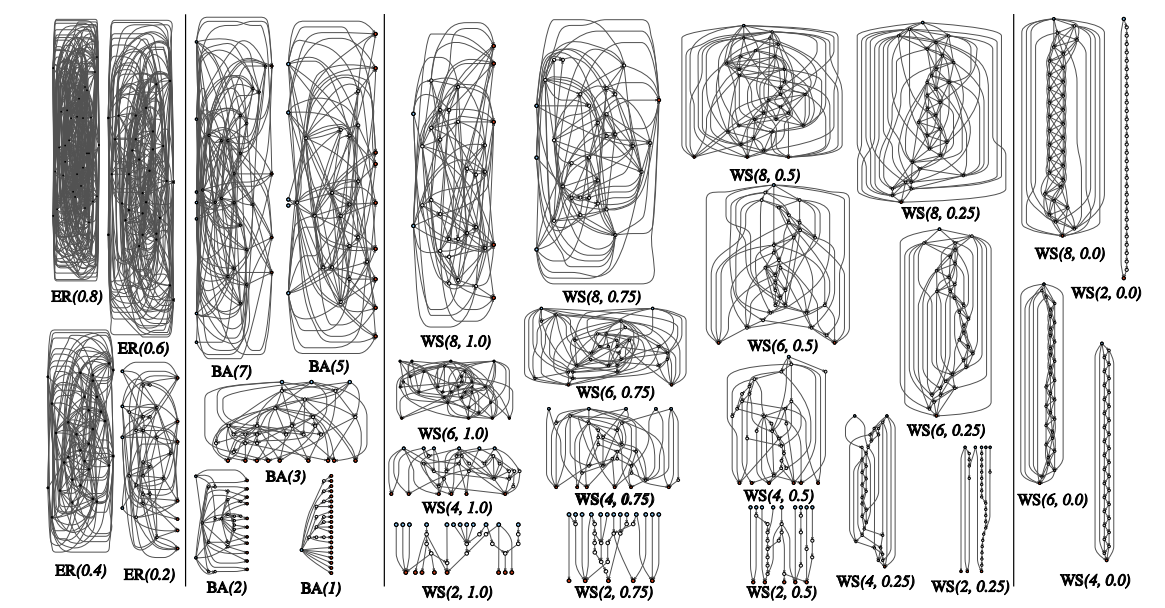
\includegraphics[width=\textwidth]{random_wiring}
    \caption[Sample random cells generated by three random graph generation algorithms]{Sample random cells generated by the three random graph generation algorithms (Erd\H{o}s-R\'enyi,
        Barab\'asi-Albert, and Watts-Strogatz).}
    \label{fig:random_wiring}
\end{figure}

These random networks are then evaluated over ImageNet, and the authors find that networks generated via the
Watts-Strogatz generator produce results that rival the state-of-the-art of both hand-designed and NAS-designed
architectures. Notably, in the sub 600M FLOP small computation regime, the Watts-Strogatz random models outperform DARTS
by 1.6 percentage points in Top-1 accuracy. The authors also look beyond raw performance, and explore the effects of different graph generators,
graph damage (defined shortly), and convolution type. For graph generators, they notice
that of the three generators used (Erd\H{o}s-R\'enyi, Barab\'asi-Albert, and Watts-Strogatz), all of them consistently
produced models that trained to decent accuracy. More interestingly, the variance of model
performance within the set of models generated by a specific generator was surprisingly low, around 0.2-0.4\%. They note
that this is only slightly larger than the variance found when retraining identical ResNet configurations, which is
between 0.1 and 0.2\%. The variance between different generators was more stratified,
with the best performing (Watts-Strogatz) a clear 3\% better than the worst, the Barab\'asi-Albert. This implies that the
broader design principles that differentiate the generators is more significant than the granular
variations between same-generator architectures. This is to say, general design parameters like the typical degree
of nodes or average path lengths through cells is more important to final performance than the minutiae of the wiring
itself.

Next they explore graph damage, the process of removing a single node or edge from a fully trained model and observing
the effects of its removal on test accuracy. Here, they compare the difference in test accuracy against the degree of the
removed node in the case of node removal, or the degree of the edge's target node in the case of edge removal. Models
generated by different graph generators had different sensitivities to this damage, with Watts-Strogatz being the
most consistently negatively affected. Specifically, Watts-Strogatz networks had a high sensitivity to the removal of
high-degree nodes and edges to low-degree nodes. The latter makes sense, as each edge to a low-degree node is more precious
than to a high-degree one and causes a greater comparative difference to that node's input. The former indicates that
these high-degree nodes act as valuable distribution hubs within this class of model. Observing the general connectivity
pattern of the Watts-Strogatz networks in Figure~\ref{fig:random_wiring} clarifies this behavior, as the high degree
nodes tend to be either the output node or are towards the end of the most significant path to the output,
while other generation algorithms tend to not have significant reliance on any single particular path. Since the Watts-Strogatz
networks are most similar to existing network design philosophies, this is useful to gain intuition as to the most
influential nodes in manual or NAS designed networks.

Finally, the authors look at changing the exact convolution schema used by the transformation nodes of the network, and evaluate
four different configurations while holding the architectures of the randomly generated networks fixed. In each of the four
configurations, the general ReLU-convolution-batch normalization stack is preserved, while the convolution is chosen
as either a 3x3 separable convolution, a 3x3 non-separable convolution, a 3x3 max pool followed by 1x1 convolution, or
a 3x3 average pool followed by 1x1 convolution. Interestingly, over 30 different random architectures the general performance
rank of the four convolution choices within the same architecture is more or less consistent,
with the separable convolution performing markedly best by around 5 percentage points over 2nd place, followed by 3x3
convolutions or 3x3 max-pools, and 3x3 average pools performing worst. Furthermore, the rank of each architecture
remains relatively consistent when convolution choice is held fixed, with the best architectures for a specific convolution
remaining among the best for different convolutions. This indicates that operation selection and architecture choice have
orthogonal effects on performance, that the best architectures will be the best architectures regardless of operation choice,
while choosing the best operations can ensure that that architecture achieves its best performance possible. This is
potentially counter-intuitive; it might be expected that different operations would prefer
specific design patterns and vice versa, however this is not the case for these random networks. This result, if it
is applicable to other network designs as well, is very useful in contextualizing comparative results between NAS algorithms.
For example, NAO uses a different operational palate than DARTS or PC-DARTS, selecting different subsets of operations
or adding in new ones depending on search constraints. Is the different performance produced by NAO to the other two algorithms
therefore a result of better architecture selection, or is due to the orthogonal performance direction of the operational palette?

Finally, the last concept that stood out from this paper is implicitly rather than explicitly introduced, and this
was removing the concept of normal and reduction cells entirely. Rather than design networks around a reduction cell
followed by a number of repeating normal cells, these networks are simply stacks of unique reduction cells.
By increasing the size of each cell, a series of cells becomes simply a possible subgraph of the larger cell, with
the exact size increase necessary to result in this behavior varying depending on the exact design philosophy of the cells.
For something like a DARTS cell with two input nodes connecting to each of the $n$ intermediate nodes and each intermediate node
connecting to each subsequent intermediate node, an $n$-node cell has $\binom{n+2}{2}-1$ edges. The ``$-1$'' term comes
from the fact that the triangular number assumes each node connects
to each subsequent node. However, input nodes only connect to intermediate nodes, which means input node 0 does not connect to input node 1.
There is therefore one fewer connection than given
by the triangular number, and thus 1 is subtracted. With this edge count, any sequence of $C$, $n$-node cells can be replaced by a single larger $m$-node cell,
such that:
\begin{align}
\binom{m+2}{2}-1 \ge C\left(\binom{n+2}{2} - 1\right). \label{eq: cell_edges}
\end{align}

In the case of n=7 and C=3 as in CIFAR-10, a single 12 node cell has
sufficient edges to be a supergraph of the original three cell stack. Furthermore, each of these larger cells is unique
in architecture compared to each other, a design feature not seen in any other cell based model thus far.

\section{Next Steps}
Intrigued by these ideas of expanding the search spaces of NAS algorithms, I wanted to apply the concepts introduced by
these randomly wired networks to NAS. Specifically, it was of interest to explore how NAS might operate over these highly unconstrained
search spaces, where each cell can be unique and the internal connectivity much more varied than any seen previously.
Doing this entailed designing a NAS algorithm that operates over an exponentially larger and more unconstrained
search space than seen in other NAS papers, and thus BonsaiNet was born.
